
\documentclass[10pt,a4paper]{report}
\usepackage{titlesec}
\usepackage[T1]{fontenc}
\usepackage{lmodern}    % prettier fonts - corrects rendering
\usepackage[utf8]{inputenc}
%\usepackage{babel}
\usepackage{float}
\pagestyle{plain}
\usepackage{graphicx}
\usepackage{listings}
\usepackage{caption}
\usepackage{gensymb}
%\usepackage{subcaption}
\usepackage{hyperref}
\usepackage[usenames,dvipsnames]{color}
\usepackage[toc,page]{appendix}

\usepackage{relsize}
\usepackage{amsmath}
\usepackage{amsfonts}
\usepackage{svg}
\usepackage{footnote}
\usepackage[textwidth=40]{todonotes}

\setsvg{inkscape = inkscape -z -D}
\graphicspath{{./},{./img/}}
\newcommand{\figref}{Rys.~\ref}

\setcounter{chapter}{4}
\setcounter{secnumdepth}{4}

\setlength\evensidemargin{0in}
\setlength\oddsidemargin{0in}
\setlength\textwidth{6.5in}
\setlength\textheight{9in}
\setlength\topmargin{0in}
\setlength\headheight{0in}
\setlength\headsep{.2in}

\renewcommand{\bibname}{References}

%zaczynaj każdą sekcję na nowej stronie
%\let\oldsection\section
%\renewcommand\section{\clearpage\oldsection}

%\title{Data flow in NEOSTEL camera \textcolor{red} {\\DRAFT \\ FOR INTERNAL USE ONLY}}
%\author{Creotech}
%\date{\today}

\begin{document}
\begin{titlepage}
\begin{center}

% Upper part of the page. The '~' is needed because \\
% only works if a paragraph has started.
\includegraphics[width=0.15\textwidth]{pict/logo.png}~\\[1cm]

\textsc{\LARGE Creotech Instruments S.A.}\\[5.5cm]

\textsc{\Large \textcolor{red} {\\DRAFT \\ FOR INTERNAL USE ONLY} }\\[0.5cm]

% Title
\hrule \textcolor{white}{test}\\[0.4cm]	%very elegant solution
{ \huge \bfseries Data flow in NEOSTEL camera  \\[0.4cm] }
\hrule \textcolor{white}{test}\\[1.5cm] %very elegant solution
 
% Author and supervisor
\noindent
\begin{minipage}{0.4\textwidth}
\begin{flushleft} \large
\emph{Authors:}\\
Marek Burza\\
Mikołaj Jamroży\\
Piotr Zdunek\\
Konrad Zgaga \\
Paweł Zienkiewicz\\
\end{flushleft}
\end{minipage}%
\begin{minipage}{0.4\textwidth}
\begin{flushright} \large
\emph{Project manager:} \\
Grzegorz Kasprowicz 
\end{flushright}
\end{minipage}

\vfill
\textsc{Version 0.1}\\[0.0cm]
% Bottom of the page
{\date{\today}}

\end{center}
\end{titlepage}

%\maketitle
\listoftodos
\tableofcontents

\chapter{Camera detailed description}

\section{Mechanical description DUMMY}

%TODO
%       ESA REMARKS:
%       Please revise document for the next major milestone (CDR?)
%       - Please describe in a top-level overview the logic of where the different functional blocks physically reside (what is central in a rack, what is on each PCB within the camera, etc.)
%       - Please describe the individual functional blocks in their logical / data flow order:
%       i) overall control of exposure sequence: camera reset, shutter, camera clocking, camera readout
%       ii) generation of top level CCD control signals; which voltages (clocks, etc.) are programmable at what level)
%       iii) generation of low-level clocking waveforms
%       iv) analog path of pixel read-out
%       v) digitized path of pixel read-out
%       vi) low-level processing of sampled pixel value (CDS, oversampling)
%       vii) "assembly" of pix values into image and data flow of image
%       - please use consistently:
%       i) exposure instead of exposition
%       ii) "housekeeping" (voltage, temp. etc.) sensors versus CCD detector chip
%TEST

%TODO Mechanizm sterowania kamerą oraz IPC skonsultować z Jackiem

%TODO - Please describe in a top-level overview the logic of where the different functional blocks physically reside (what is central in a rack, what is on each PCB within the camera, etc.)
\section{Camera Electronics - Architectural Overview and Subsystem Decomposition}
%Jeśli opisujemy w stylu report tzn. jako rozdziały i sekcje
%to warto dawać wstęp na poczatku każdego rozdziału  Piotr Zdunek
%Może jednak zrobimy same sekcje, bez rozdziałów?

\subsection{Introduction}

The electronics of the Camera Assembly consist of two main parts. First is the Control and Communication Board and second is the Mainboard with Analog Front-End (AFE), Detector, Power Supply and Driver Modules. 
Principal parts and functions of the boards and modules are presented within the block diagram of \ref{fig:cam_overview}. 

\begin{figure}[H]
\centering
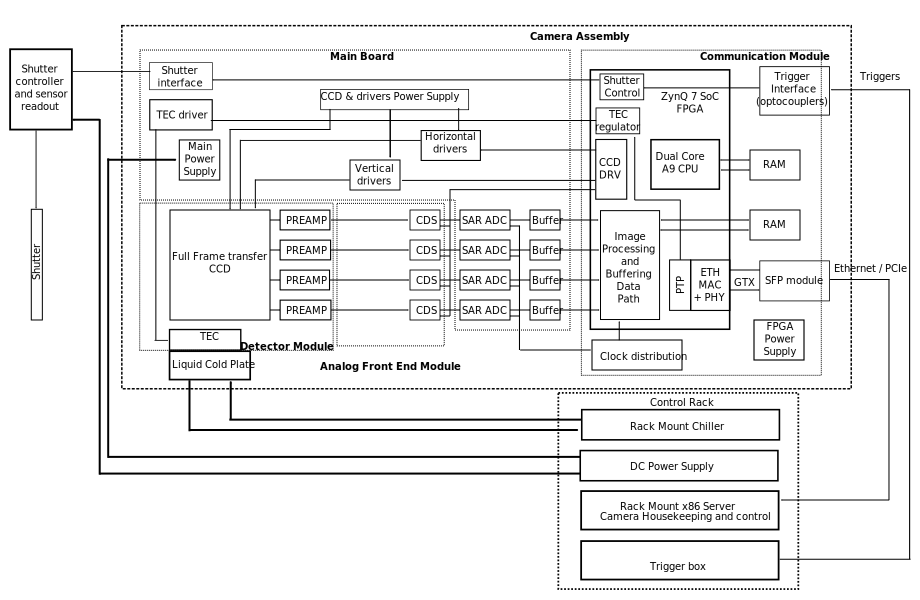
\includegraphics[width=\textwidth]{pict/cam_overview.png}
\caption{NEOSTEL camera block diagram}
\label{fig:cam_overview}
\end{figure}

The processing platform of the Control and Communication Board is based on a Xilinx Zynq System-on-Chip (SoC) solution that includes a two-core Cortex A9+ application processor and one Field-Programmable Gate Array (FPGA). It also contains a number of integrated peripheral interfaces like Ethernet, SPI, I2C, CAN, USB etc. as well as two DDR3 memory controllers. 
The system runs both Linux and RTOS operating systems in an AMP scenario, with Linux being responsible for the high level control and maintenance and with RTOS being in charge of time critical tasks. The entire communication is based on the Ethernet interface. A PTP synchronization protocol provides a microsecond synchronization capability. A serial port is used as standard console output for diagnostic purposes.
The Mainboard integrates controllers for the analogue front-end, CCD sensor (detector) TEC module, diagnostics and sensors.
The system is controlled via EPICS and provides server functionality. Image data will be double buffered and sent to a remote facility server in FITS format.

\subsubsection {Electronic System Features}
\begin{itemize}
\item Low noise 16MP CCD sensor readout – images are handled in a self-describing FITS format with additional diagnostic information
\item Shutter control with accurate start/stop position feedback implemented in the FPGA in the external shutter module
\item Environment measurements (humidity, temperature, position)
\item EPICS SCADA support with EPICS server implementation for system diagnostics and control
\item High speed interface: 1 Gbps Full Duplex Ethernet through SFP transceivers with full hardware PTP support including time-stamping
\item Internal and external trigger
\item Time synchronization via PTP
\item Heterogeneous system with both RTOS (for time-critical procedures) and Linux (for interfacing flexibility and easy data processing with low latency control and a diagnostics path)
\item Universal CCD data readout with flexible FPGA logic and modular AFE
\item Innovative Xilinx Zynq SOC design with dual core Cortex A9+ and FPGA on one silicon DIE with shared subsystems.
\end{itemize}

\subsection{Camera modules location within camera}
Camera modules location within camera is presented in figure x.x in mechanical description of camera.

\subsection{Control and Communication Board}

A Communication Board block diagram is presented in figure \ref{fig:commbrd}.

\begin{figure}[H]
\centering
\includegraphics[width=\textwidth]{pict/commbrd_block.png}
\caption{Communication board block diagram}
\label{fig:commbrd}
\end{figure}

The Communication Board connects with the Mainboard. It is an interface between camera electronics and an external server. The role of this board is:
\begin{itemize}
\item The generation of timing signals for the CCD sensor
\item The generation of timing signals for the Analog Front-End module
\item The data collection from analog-to-digital converters and sensors
\item The communication via Ethernet
\item The time synchronization using a PTP protocol.
\end{itemize}

The main processing unit is a Zynq SoC, containing a two core ARM Cortex A9+ processor and the FPGA logic. This part supervises all onboard peripherals and CCD sensor operations. It also sets the proper voltage to supply and bias the CCD, drives the CCD signals, receives data from A/D converters and sends data via the Ethernet. The Zynq processor has been chosen due to its ability to support 1 or 10 Gbit Ethernet. 

The Zynq SoC uses two types of the memory. The first one is volatile (RAM) memory; the second one is non-volatile (FLASH) memory. The RAM memory keeps the data and is required for image processing purposes, whereas the FLASH memory contains the Linux file system. There is an additional storage device on the module - a Micro SD card is used to store system logs.

The Ethernet connection is established by a SFP/SFP+ transceiver. Thus a copper or optical Ethernet connection can be implemented. The internal power supply consists of two quad channel high efficiency DC/DC converters that supply all devices on the module. A detailed electrical scheme is presented in the mainboard file.
\todo[inline, caption={Datapath}]{Co to jest mainboard file}
\subsubsection{ZYNQ SOC}
The ZYNQ SoC manufactured by Xilinx is the most important part of the communication module. The XC7Z030-2FFG676I chip was chosen because of the four high speed transceivers implemented in the 676-ball BGA package.
It has two so-called high-range (HR) banks, three high-performance (HP) banks, processing system (PS) banks and a single high-speed GTX transceiver bank. HR, HP and GTX banks belong to the FPGA of the SoC. The PS banks belong to the processor part of the SoC.
Pins from HR banks drive UART, SPI, IIC, LVDS and MLVDS interfaces. There are also general-purpose pins to drive LEDs and to check the state of the push-button switches.
HP banks are used as an interface to the SDRAM DDR3 memory and as a LVDS interface.
PS banks are the ARM processor external interface. They are connected to the SDRAM DDR3, NAND Flash, NOR Flash and SD card. Some of the pins are general-purpose pins and drive LEDs and interfaces like IIC, SPI, CAN and UART. The ARM processor can boot from all non-volatile memories mentioned above. 
A general block diagram of the ZYNQ 7000 SoC is shown in figure \ref{fig:zynq} (Source: www.xilinx.com).

\begin{figure}[H]
\centering
\includegraphics[width=0.7\textwidth]{pict/zynq.png}
\caption{ZYNQ SOC block diagram}
\label{fig:zynq}
\end{figure}

\subsubsection{Clock generators}

There are five oscillators on the Communication Board \ref{tab:clocks}. Two of them are ARM system clocks; the other three drive GTX interfaces.

\begin{table}[]
\centering
\caption{Clock generators}
\label{tab:clocks}
\begin{tabular}{|l|l|l|l|}
\hline
Oscillator part number & Frequency & Connected to & Role \\ \hline
SiT8103AC-32-18E-33.33300X & 33,33 MHZ & ARM & System clock \\ \hline
570BBC000121DG & 10-280 MHz & ARM & RAM clock \\ \hline
ASFLMPLV-156.250MHZ-LR-T & 156,25 MHZ & FPGA & 10 Gbit Ethernet clock \\ \hline
LF VCXO026156 & 20 MHz & FPGA & White Rabbit clock \\ \hline
VM53S3-25.000-2.5/-30+75 with CDCM61004RHBT & 125 MHz & FPGA & White Rabbit clock \\ \hline
\end{tabular}
\end{table}

\subsubsection{VOLATILE MEMORY}
The Communication Board contains two banks of SDRAM DDR3 memory. Each bank contains two 16-bit 128Mx16 chips. The first memory group is controlled by the FPGA, the second by the ARM processor. The single memory chip has a capacity of 2Gb (512 MB). 

\subsubsection{NON-VOLATILE MEMORY}
There are three types of non-volatile memory on the Communication Board. The first one is a NAND Flash, ONFI compatible. The MT29F8G08ABBCAH4 memory was chosen. It is a single chip, 8Gbit (1GB), 8-bit NAND memory, to store the Linux file system.
The operating system data can also be stored into a NOR Flash. Two S25FL128SAGMFIR01 chips are used. A single one is a 128Mbit (16MB) Flash memory chip with a fast quad-SPI interface. 
The third memory is a micro SD card (user defined capacity). The TXS02612RTWR level translator is placed between the SoC and the SD card.
The Zynq Soc can boot from all of these memories. Boot-mode can be selected by using jumpers.
\todo[inline, caption={Datapath}]{Ten akapit w kilku miejscach jest mało logiczny}

\subsubsection{SEARAY CONNECTOR}
Searay connector (SEAF-20-01-X-10-X-RA) connects with the Mainboard. It delivers supplies and MLVDS and LVCMOS interfaces to the rest of the electronic circuitry.

\subsubsection{MINI-SAS CONNECTOR}
A Mini-SAS connector is optional and can be used in the future. It is electrically connected to the Zynq GTX transceivers. Thus PCIe x4 or 40Gbit Ethernet can be implemented.
\subsubsection{USB}
A user-friendly debugging interface is implemented. There are two CP2102-GM USB-to-UART bridges connected to the FPGA part of the SoC.
The detailed electrical schematic is presented in the USB.SchDoc-file.

\subsubsection{SFP+}
One GTX transmitter and one receiver of the SoC are connected to the SFP+ module. This has been chosen such due to the ability to transceiver fast 1 and 10 Gbit signals used in Ethernet connections. The resistor tree provides backward compatibility with the SFP module.
The detailed electrical scheme is presented in the SFP+.SCHDoc-file.

\subsubsection{RS485 AND OPTO-INTERFACE}
These interfaces are used for trigger and shutter control. The RS485 is bi-directional; the opto-interface has four inputs.

\subsubsection{Power supply}
The power supply chain of the Communication Board is presented in the block diagram of figure \ref{fig:powersup}.

\begin{figure}[H]
\centering
\includegraphics[width=\textwidth]{pict/power_supply.png}
\caption{Power supply chain of the Communication Board}
\label{fig:powersup}
\end{figure}


P12V0 is the main power supply from the external power adaptor. There are two quad synchronous buck converters that convert the main supply into several voltages. Each converter channel consists of a common controller/driver (XRP7724) and of external high-power transistors (STL60N32N3LL). P1V2, P1V6, P2V9, and P5V0 rails supply the mainboard through a Searay Connector. Other voltages from a second DC/DC converter, P1V0, P1V5, P1V8, and P3V3 supply the SoC, some peripherals, and LDOs. LDOs are used to supply noise-sensitive parts e.g. SoC GTX transceivers or the DDR3 reference voltage. 
Detailed electrical schemata are presented in the Power.SchDoc-, Power supply linear.SchDoc- and Power supply switching.SchDoc-files. 
Shutter interface and trigger signals will be delivered using standard Amphenol, M12 ruggedized connectors.
The layout of the Communication Board is presented in Figure 5 39.

\begin{figure}[H]
\centering
\includegraphics[width=\textwidth]{pict/commbrd_layout.jpg}
\caption{Layout of the communication board}
\label{fig:commbrd_layout}
\end{figure}

\subsubsection{LAN interface and data link transfer aspects}
A SFP+ cage (Small Form-factor Pluggable Transceiver) provides the communication interface of the camera. Several types of optical or copper transceivers will be installed. Gigabit Ethernet or even PCI Express Gen II protocols can be used without hardware modifications.
To enable the communication between several cameras, Gigabit Ethernet and a TCP protocol are implemented. This provides for each camera the option of a fully autonomy control and data acquisition. Since each camera has an independent operating system, the measurement data (FITS files) can be stored directly using NFS or FTP protocols on suitable servers.
The main system architecture data path starts at the CCD sensor readout (16 ADCs) and ends at the FPGA fabric on the Zynq SoC. The Data can be read from the sensor and sent to the processing system in real time. The latter packages the data into FITS format and sends the according FITS files to the control system (PC server) via a Gigabit Ethernet interface (Figure 5 40). Gigabit Ethernet is implemented by means of a GTX transceiver and PCS/PMA logics. It cooperates with a hardcoded MAC block that is directly connected to the ZynQ CPU subsection.
The AFE produces 16 serial streams of 100Mbit/s each. These streams are de-serialized by the IP Core and transferred by the AXI stream to the ZynQ memory.

\begin{figure}[H]
\centering
\includegraphics[width=\textwidth]{pict/datapath.png}
\caption{Datapath}
\label{fig:datapath}
\end{figure}

\todo[inline, caption={Datapath}]{Poprawić, bo rysunek ma błędy}

\subsection{Main Board}

\begin{figure}[H]
\centering
\includegraphics[width=\textwidth]{pict/mainbrd.png}
\caption{Main Board block diagram}
\label{fig:mainbrd}
\end{figure}

Figure \ref{fig:mainbrd} provides the block diagram of the systems connected to the Mainboard. Analog Device ADC (AD7960) 18bit SAR converters have been selected due to their low noise abilities, high SNR, and relative high sampling rate. Four ADCs will be implemented to sample each CCD channel – the goal is to oversample the signal and to utilize a digital signal processing to filter white and correlated noise. To lower the jitter of the sampling clocks, an additional buffer will be used that distributes the signal point-to-point.
The Analog-Front-End (AFE) board contains a circuitry designed to process raw analogue data from the CCD matrix. Depending on its implementation it can be CDS or adaptive filtering and buffering of the input signal. Several implementations are considered and the one with best noise characteristics will be chosen for the final version of the camera.
The Shutter driver is enclosed in the shutter case and implemented as a linear amplifier with a current limiter (through feedback), working in a half bridge configuration. The position detection of the shutter blades is provided by dedicated sensor. It is connected with the Mainboard using a sealed connector where RS485, I2C, and logic control signals are distributed.
The Mainboard also contains the Peltier Thermoelectric Cooler (TEC) with a half bridge driver set trough a PWM controller. An additional feedback circuit is used on the board to measure the current of the Peltier module. The PWM operation is synchronized with the CCD operation to prevent noise interference propagation to the AFE chain.
The board also has a dedicated ADC for reading the PT-1000 temperature sensors that measure the temperature in different parts of the camera. 

\subsubsection{CCD and CCD driving signals}
The main task of the camera Mainboard is to provide power to all other modules of the camera - generated from one single standard 24V power entry and the CCD control.  All voltages needed by the detector module - power, bias, reset and clocking upper and lower levels - are adjustable by Digital-to-Analog Converters (DACs). The programmable range fits within the safety region defined by the sensor manufacturer.
The sensor is critical part of the design. Therefore, the NEOSTEL camera was designed to support at least two different CCD vendors – E2V and Andanta, given the possibility that one CCD prototype could not be available at the time of deployment. A third vendor, Fairchild Imaging does not produce suitable sensors anymore. Table \ref{tab:CCD} summarizes the parameters of three foreseen sensors.
The E2V sensor is described by the manufacturer in a substrate biased configuration at positive level (instead of ground) to enable positive voltage biasing and clocking. However, a bipolar operation was selected, with the substrate connected to the ground to preserve similar supply and driving circuits for both sensors. The resulting bias voltages corrected all driving and biasing voltages specified by the manufacturer. Thanks to this approach, similar voltage levels can drive both sensors and differences can be compensated by means of resistive dividers at LDO regulators. \\
When it comes to the CCD sensor decision, E2V CCD231-84 is considered as a better solution while Andanta CCD4150A is the backup one. CCD231-84 provides a better dark current noise characteristic, which is one of the key parameters for the camera. An additional advantage over the alternative sensor is that it has additional inputs that allow for a faster binning and cleanup process.

\begin{savenotes}
\begin{table}[!htbp]
\centering
\caption{CCD comparison}
\label{tab:CCD}
\begin{tabular}{|c|c|c|c|c|}
\hline
 & CCD4150A & CCD230-84 & CCD231-84 & Units \\ \hline
Manufacturer & Andanta & E2V & E2V & \\ \hline
Operation mode & NIMO/MPP & MPP & NIMO & \\ \hline
Resolution &4096 x 4096 & 4096 x 4096  & 4096 x 4096 & pix \\ \hline
Pixel size & 15 x 15 & 15 x 15  & 15 x 15 & $\mu$m \\ \hline
Image Area &61.44 x 61.44& 61.44 x 61.44 & 61.44 & mm \\ \hline
Illumination & Backside & Backside & Backside &  \\ \hline
Clocking sequence & three--phase& four--phase & four--phase &  \\ \hline
Outputs &4& 4 &4 &  \\ \hline
Fill factor &near 100& near 100 &  near 100 & \% \\ \hline
Maximum rate of heating or cooling & N/A & 5 & 5 & K/min \\ \hline
Dark current & 5.0 $\frac{e^{-}\cdot h}{pix}$ (163K) &2.0 $\frac{e^{-}\cdot s}{pix}$ (248K)&  0.2 $\frac{e^{-}\cdot s}{pix}$ (153K) & \\ \hline
Image FWC (NIMO/MPP)  & 300k/150k &  NA/150k & 350k/NA  & $e^{-}$ \\ \hline
Output FWC (OG mode)  & TBD  & 450k/900k & 200k/600k & $e^{-}$ \\ \hline
Output amplifier sensitivity & 5 & 2.5 & 7 & $\mu V/e^{-}$ \\ \hline
Output rms noise  & 2.5 (@100kHz)  & 4 (@50kHz) & 2 (@50kHz) & $ e^{-}$ \\ \hline
Charge transfer efficiency & >99.999 &  >99.999 &  >99.999 & \% \\ \hline
Spectral range & 300--1060 & 300--1060 & 300--1060 & \% \\ \hline
Minimum full frame read time & & 1.064 & 1.531 & s\\ \hline
Minimum full frame dump time &  & 0.256 & 0.179 & s\\ \hline
ROI (512x512 pix) read time \footnote{Details described in section \ref{sec:windowing}} & & 0.377 & 0.360 & s\\ \hline
\end{tabular}
\end{table}
\end{savenotes}

The CCD sensor requires several bias voltages that are generated by low noise – Low Drop Out (LDO) regulators that are trimmed by DACs.
The CCD drivers require a low ripple and stable power supply. Therefore, all needed power voltages are provided by LM1117/LM337 LDO and linear regulators that are trimmed by DACs. The industrial temperature range for all semiconductors was chosen.
For the horizontal and vertical transfer electrodes, EL7457 drivers are used. At the output of these drivers, resistors are installed that limit dv/dt. A too high dv/dt would cause charge efficiency degradations. \\
Control signals for CCD drivers as well as AFE are generated by Pattern Generator \ref{sec:patgen} IP-core within FPGA on Communication Board. 16 ADCs are dedicated for readout of the CCD data. \\

\subsection{Hardware monitoring sensors}
All of camera PCBs are equipped with various sensors including temperature, humidity, voltage sensors, accelerometer and tachometer. Function of the accelerometer is to detect vibrations caused by e.g. the shutter. Some sensors located in critical parts of the camera have capability of hardware monitoring and power shutdown. \\
List of sensors used in the camera is presented below:

\begin{description}

\item \textbf{Communication board} \hfill \\
\begin{itemize}
\item voltages
\item humidity
\item 2x temperature
\end{itemize}

\item \textbf{Mainboard} \hfill \\
\begin{itemize}
\item humidity
\item temperature
\item 3x temperature
\item acceleration (3-axis)
\item coolant volumetric flow rate - tachometer
\end{itemize}

\item \textbf{CCD board} \hfill \\
\begin{itemize}
\item humidity
\item temperature
\end{itemize}

\item \textbf{Shutter} \hfill \\
\begin{itemize}
\item humidity
\item temperature
\end{itemize}

\end{description}

\subsection{Shutter electronic design}

\subsubsection{Introduction}

The Electronics of the shutter is placed inside the shutter’s replaceable module. It contain an FPGA that controls the shutter mechanism and receives the information of the shutter position from the position sensors.

Figure \ref{fig:shutconn} shows the connection between camera and shutter modules. The shutter can also be controlled via RS485 or analog trigger signals. The trigger signals (ACTION) for each shutter module are opto-isolated and available on the back panel of the camera. Output signals (CONFIRM) are asserted when correct shutter opening or closing occurs.
The I2C bus is used only to upload an FPGA firmware directly from camera. It is connected to flash memory from which the FPGA download it's firmware.

\begin{figure}[H]
\centering
\includegraphics[width=1\textwidth]{pict/shutter_connection.png}
\caption{Shutter-camera connection block diagram}
\label{fig:shutconn}
\end{figure}

Shutter electronic module contains: motor driver, two blade position sensors, temperature and humidity sensor and accelerometer. Figure \ref{fig:shutblk} presents the block diagram of the shutter’s module internals. 

\begin{figure}[H]
\centering
\includegraphics[width=1\textwidth]{pict/shut_block.png}
\caption{Shutter's module block diagram}
\label{fig:shutblk}
\end{figure}

\subsubsection{Position sensor}

For the precise knowledge about the exact position of the shutter blade(s) during opening and closing, a high precision encoders signals is recorded and timestamped. Shutter is equipped with 2 position sensors, one absolute and one incremental.

The absolute shutter positioning system is based on a capacitance measurement. Sensor have two capacitors that are made of PCBs with copper plate. Capacity of those capacitors (C1 and C2 on \ref{fig:shutsens}) is changing during movement of the blade: one increase his capacity and the other decreases it (and the other way during movement in the opposite direction). One can change the differential capacity to the coroleted voltage output, so it is possible to plot the voltage vs blade position characteristic. Detailed description of sensor design is in 5.1.6.3 subsection.

To translate a capacity to voltage a high frequency generator is connected to capacitors – leading to output's DC component linearly depends on the capacity. This signal is filter to get only DC component, then it is amplified to get the best dynamic range and then it is measure by ADC. \ref{fig:shutsens}.

\begin{figure}[H]
\centering
\includegraphics[width=0.9\textwidth]{pict/shut_sens.png}
\caption{Shutter's capacity position sensor schematic}
\label{fig:shutsens}
\end{figure}

Second position sensor is the incremental magnetic sensors RLS RLC2IC. Sensor has 3 differential lines as an output 'A','B' and 'Z'. 'A' and 'B' signals creates the incremental quadrature pair that give a pulse after every 5um of displacement. Quadrature encoding give a possibility to detect the direction of the moment. 'Z' signal give reference pulse each 2mm \ref{fig:shut_mag_sens_wave}. These signals are feed to differential line receiver (DS26LV32AT) to change signal to LVCMOS level to be compliant with FPGA inputs \ref{fig:shut_mag_sens_sch}.

\begin{figure}[H]
\centering
\includegraphics[width=0.7\textwidth]{pict/shut_sens_magnetic.png}
\caption{Shutter's magnetic position sensor schematic}
\label{fig:shut_mag_sens_sch}
\end{figure}

\begin{figure}[H]
\centering
\includegraphics[width=0.7\textwidth]{pict/shut_sens_magnetic_waveform.png}
\caption{Shutter's magnetic position sensor waveform}
\label{fig:shut_mag_sens_wave}
\end{figure}

\subsubsection{Driver}
Each shutter motor has an independent driver, allowing controlling the movement of each blade. The separation of the individual channels allows a synchronization of the speed of both blades despite the differences in the direction of the gravitational force. The diagram below shows one single shutter driver channel.

\begin{figure}[H]
\centering
\includegraphics[width=0.7\textwidth]{pict/shut_drv.png}
\caption{Shutter driver (actuator)}
\label{fig:shutdrv}
\end{figure}

A single SPI Digital to Analogue Converter (DAC) with two independent analogue outputs (DAC7612) controls the shutter driver channel. To provide the motors with sufficient current, an additional differential buffer is used. This buffer is implemented on OPA548 operational amplifiers with an output current up to 5A. The buffers have an implemented thermal shutdown to protect the shutter driver from overheating. Buffers are connected to output headers by LC PI-type filters to minimize the EMI.
The positive output of the differential buffer is connected to a current monitor, which is implemented as a 10MOhm resistor with an AD8031 operational amplifier, set to a gain of 20. The output of the current monitor is connected to an ADS7945 SPI SAR 14-bit ADC and creates a feedback path. This solution allows implementing control algorithms that can modulate the DAC output to accomplish a constant current drive instead of a constant voltage.
Two modes of shutter driver operation are being considered – an operation with feedback from the shutter positioning subsystem or an operation based on lookup tables. In the first solution, a digital controller e.g. PID is feed with the shutter position and the motor drive current. This allows the adjustment of the speed of the blade. In the second solution, a table of drive values is created, based on calculations and adjusted by experiments. The table will contain a set of analogue values for the DACs that will be applied within a specific time interval to obtain a repeatable shutter movement.
\subsubsection{Sensors}

Each shutter module is equipt with addition sensors:
\begin{itemize}
\item Temperature and Humidity (HDC1000) - detecting the overheat of the shutter's electronic and measuring the humidity around the camera window to predict the window heater work.
\item Accelerometer (ADXL343) - measure vibration generated by shutter
\end{itemize}

\subsubsection{Control}
%\todo[inline, caption={Failsafe shuttera}]{ Schemat nie uwzględnia co robimy w przypadku %błędu, żadnego failsafe/override dla procedury. To jest mechanika, jeśli error to %zostawiamy shutter wiszący w połowie? W jaki sposób jest przewidywana sygnalizacja stanów %i w jaki sposób jest przewidywana obsługa otoczenia shuttera w każdym z nich? /PZi}

Each Shutter module interface contains:

\begin{itemize}
\item Action line (input) - triggering opening or closing of the blade
\item Confirm line (output) - confirmation of opening or closing of the blade
\item RS485 bus (slave) - communication between camera and shutter module
\end{itemize}

RACZJE USUNAC TEN OBRAZEK NIŻEJ
\begin{figure}[H]
\centering
\includegraphics[width=0.7\textwidth]{pict_ipc/shutter_control.png}
\caption{Shutter internal control state chart}
\label{fig:shutctrl}
\end{figure}

For system point-of-view shutter control description refer to section \ref{sec:shutctrl}.

\paragraph{Shutter control signals waveforms}

The motion of the blade is triggered by rising edge of the ACTION line. The ACTION line has to by 'HIGH' for at least 10us for shutter to trigger the event, this is to ensure that debouncing mechanism don't discard the pulse as a glitch. 
When event occurs, shutter starts moving the blade and recording motion data. When the movement of the blade is finished the CONFIRM line change to 'high', which is a signal to the camera that shutter opening or closing is 
completed. The ACTION line toggle the current shutter state, so the normal operation during taking picture is to pulse the ACTION line to open the shutter, then after the exposure time pulse it again to close the shutter blades.

Each shutter module has it own ACTION and CONFIRM line, the RS485 bus is in multi-drop configuration with camera as a master and two shutter module as a slaves. The CONFIRM line is used to ensure that each shutter blade did it action correctly. The CONFIRM line 
stay 'high' until the shutter module received a reset command via RS485. The ACTION line don't trigger any action before the shutter is not reset. During the reset, all the capture motion data are erase, so the normal operation will be to first read those data, then reset the shutter. The waveform diagram below shows the typical shutter operation during image acquisition.

\begin{figure}[H]
\centering
\includegraphics[width=1\textwidth]{pict/Sht_Wafeform.png}
\caption{Shutter interface waveform for opening and closing}
\label{fig:shtwf}
\end{figure}

During the movement the motion data are analysed and the errors are detected.
Below is a shutter module state diagram.

\begin{figure}[H]
\centering
\includegraphics[width=0.7\textwidth]{pict_ipc/Sht_FSM.png}
\caption{Shutter stage diagram}
\label{fig:shtfsm}
\end{figure}

From shutter point of view, there is no difference between external (diagnostic mode) and internal control.

\paragraph{Communication protocol} 
%\\newline
Shutter communicate with the camera via RS485 interface. Camera is a master and two shutter modules are slaves that only can respond to command, they can't start the transmission. CRC is used as an error-detecting method, if the error is detected the receiver send a error code and data frame is retransmitted.


Each data frame sent from camera to shutter contains:
\begin{itemize}
\item Start frame (1 byte)
\item Slave adress  (1 byte)
\item Command code (1 byte)
\item Data bytes (optional - depends on command)
\item CRC bytes  (2 byte)
\item Frame end byte (1 byte)
\end{itemize}

Each data frame sent from shutter to camera contains:
\begin{itemize}
\item Frame start byte (1 byte)
\item Data bytes (depends on command)
\item CRC bytes (2 byte)
\item Frame end byte (1 byte)
\end{itemize}

	\begin{table}[H]
\begin{center}
    \begin{tabular}{| l || l  || l  |}
    \hline
    \bf{Command}				& \bf{Code (hex)} & \bf{Respond}\\ \hline
	Reset						& 0  		 	  & ACK / NACK	\\ \hline
	Send motion data			& 11  		 	  & data 		\\ \hline
	Send temperature			& 12  		 	  & data		\\ \hline
	Send humidity				& 13  		 	  & data		\\ \hline
	Send acceleration			& 14  		 	  & data		\\ \hline
	Send coil current			& 15  		 	  & data		\\ \hline
	Send absolute position		& 16  		 	  & data		\\ \hline
	Send incremental position	& 17  		 	  & data		\\ \hline
	Error						& 2  		 	  & Error code	\\ \hline
	Open shutter				& 31  		 	  & ACK / NACK	\\ \hline
	Close shutter				& 32  		 	  & ACK / NACK	\\ \hline
	Move to position			& 33  		 	  & ACK / NACK	\\ \hline
	Send status					& 4  		 	  & Status code	\\ \hline
	Shutter emergency shutdown 	& 5  		 	  & -			\\ \hline
	Retransmission request 		& 6  		 	  & depend		\\ \hline
    \end{tabular}
    \end{center}
    \caption{Shutter command list}
	\label{table:shut_err_table}
\end{table}

	\begin{table}[H]
\begin{center}
    \begin{tabular}{ | l || l  |}
    \hline
    \bf{ACK/NACK}		& \bf{Code} 	\\ \hline
	Acknowledge			& 0 	\\ \hline
	Non Acknowledge 	& 1 	\\ \hline
    \end{tabular}
    \end{center}
    \caption{Shutter acknowledge coding table}
	\label{table:shut_err_table}
\end{table}
	
	\begin{table}[H]
\begin{center}
    \begin{tabular}{ | l || l  |}
    \hline
    \bf{Error} 							& \bf{Code} 	\\ \hline
	No problem							& 0 	\\ \hline    
	Shutter mechanical problem			& 1 	\\ \hline
	Shutter overheat					& 2 	\\ \hline
	Shutter unknown error				& 3 	\\ \hline
    \end{tabular}
    \end{center}
    \caption{Shutter error coding table}
	\label{table:shut_err_table}
\end{table}

	\begin{table}[H]
\begin{center}
    \begin{tabular}{ | l || l  |}
    \hline
    \bf{Status}				& \bf{Code} 	\\ \hline
	Shutter open			& 0 	\\ \hline
	Shutter closed			& 1 	\\ \hline
	Shutter during motion	& 2 	\\ \hline
	Shutter motion finished & 3 	\\ \hline		
	Shutter fail 			& 4 	\\ \hline
    \end{tabular}
    \end{center}
    \caption{Shutter status coding table}
	\label{table:shut_err_table}
\end{table}

\subsection{CCD cooling subsystem}

\subsection{Camera time synchronization mechanism}
\subsubsection{Introduction}

The following actions of the camera are time-stamped:
\begin{itemize}
\item Trigger event
\item Start of shutter opening
\item Start of shutter closing
\item Start of CCD readout
\item Arming camera
\end{itemize}

The figure below \ref{fig:ptptopo} presents a scheme of the PTP synchronization subsystem. Each camera as well as processing server is connected to a common Gigabit Ethernet Switch with PTP capability. A PTP time master is used to distribute the time to the entire NEOSTEL installation.

%Dodane Pzi:
\todo[inline, caption={PTP - szerszy opis, doprecyzowanie}]{Opisac pobieżnie mechanizm synchronizacji PTP, również w przypadku używania w serwerach standardowych x86 - jest dobry dokument Fujitsu o tym - http://events.linuxfoundation.org/sites/events/files/slides/lcjp14\_ichikawa\_0.pdf jest to standard w przypadku rozproszonych tranzakcyjnych baz danych. W NEO, jeśli daemon PTP będzie działać to bierzemy wersję z HW TSTAMP i mamy wszystkie mechanizmy opisane w dokumencie (łącznie z phc), trzeba będzie na koniec sprawdzić implementację PTP pod kątem: działania na warstwie 2, warstwie 3, po TCP, UDP i IPv6.
PTP Time synchronization with the same algorithm will be used in every Neostel Camera server providing common time for all of the system./ PZi}

\begin{figure}[H]
\centering
\includegraphics[width=0.6\textwidth]{pict/ptp_topo.png}
\caption{PTP synchronisation network topology}
\label{fig:ptptopo}
\end{figure}

Utilizing NTP is also possible, using the standard Linux daemon service.
We are considering 2 possible PTP synchronisation solutions: one using built-in MAC and the other using dedicated PL IP core. Both solutions are described in detail below.

\subsubsection{Integrated MAC solution}

\begin{figure}[H]
\centering
\includegraphics[width=0.7\textwidth]{pict/soft_ptp.png}
\caption{PTP timestamping using integrated MAC PTP HW and Linux PTP driver}
\label{fig:softptp}
\end{figure}

The PTP synchronization schematic using built-in MAC is presented on figure \ref{fig:softptp}.
The ZynQ SoC Media Access Controller block is PTP-capable, including hardware packets timestamping. PTP synchronization is provided by dedicated Linux driver in cooperation with PTP-capable hardware in MAC. PTP time is kept in specialized, memory-mapped hardware register in MAC.  Microsecond synchronization accuracy is possible. \\
Camera event timestamping is implemented in software in each event's ISR. Each event triggers appropriate interrupt in CPU Core 1 (RTOS). Each event's ISR reads the time-stamp value from the PTP Ethernet register in MAC and assigns it to that specific event. Such solution is a compromise between complexity and accuracy, because the ZynQ does not provide direct hardware access to the time-stamp register in PTP MAC. Because interrupts are serviced on RTOS, both low jitter and delay are expected (sub-10 $\mu s$ range).

\section{Camera video frame acquisition flow description}

\subsection{Introduction}
This chapter presents camera electronic hardware and firmware structure in data-flow, bottom-to-top order. 
Description starts with analogue subsystem (AFE) and low-level digital subsystem ADC interface and ends with operating system and high-level camera control.

%TODO - Please describe the individual functional blocks in their logical / data flow order:
%       i) overall control of exposure sequence: camera reset, shutter, camera clocking, camera readout
%       ii) generation of top level CCD control signals; which voltages (clocks, etc.) are programmable at what level)
%       iii) generation of low-level clocking waveforms

\subsection{Overview}
Figure \ref{fig:adciface} presents general block structure of Neostel camera dataflow and control. For clarity, external or auxiliary modules such as shutter and Peltier cooling controllers are not shown here. Overall structure is as follows: CCD sensor is connected through AFE and ADCs to the Zynq SOC. All control signals for the CCD and ADCs are generated by \emph{Pattern Generator} core inside Zynq Programmable Logic. Signals outgoing from FPGA are resynchronized in \emph{Input-Output Blocks} (IOBs). CCD sensor digital front-end is clocked with independent, external, low jitter clock. Along with CCD and ADC control signals, video synchronization signals for \emph{ADC interface} are generated. The \emph{ADC interface} is responsible for reading sampled data from the ADC, processing these data into pixels, and sending the data along with synchronization signals to the \emph{Direct Memory Access engine} core. DMA engine then writes video frame to DDR memory. The Zynq SOC is equipped with two independent DDR memory banks – the first bank, connected to Processing System; the second bank to the Programmable Logic. DMA can be configured to write to either of these locations. Default destination for the CCD data is PS memory but for the debug and development purposes it can be switched to the PL memory. \\
Next steps of data flow are executed by the software running on ARM Cortex A9 APU. Video frame is read, reordered and formed into FITS format image. Ready image is then forwarded to the \emph{EPICS} facility control system and sent out to the client. \\
All of the main processing blocks are connected with AXI bus and can be individually programmed and controlled by software. Hardware trigger is provided by \emph{Trigger IP} - which forwards external trigger or can be released by software. Trigger IP is also connected to the \emph{Global Interrupt Controller}.

\begin{figure}[H]
\centering
\includegraphics[width=0.8\textwidth]{pict/adc_interface.png}
\caption{Neostel camera IP structure overview}
\label{fig:adciface}
\end{figure}

\subsubsection{Pattern generator}
\label{sec:patgen}

\begin{figure}[H]
\centering
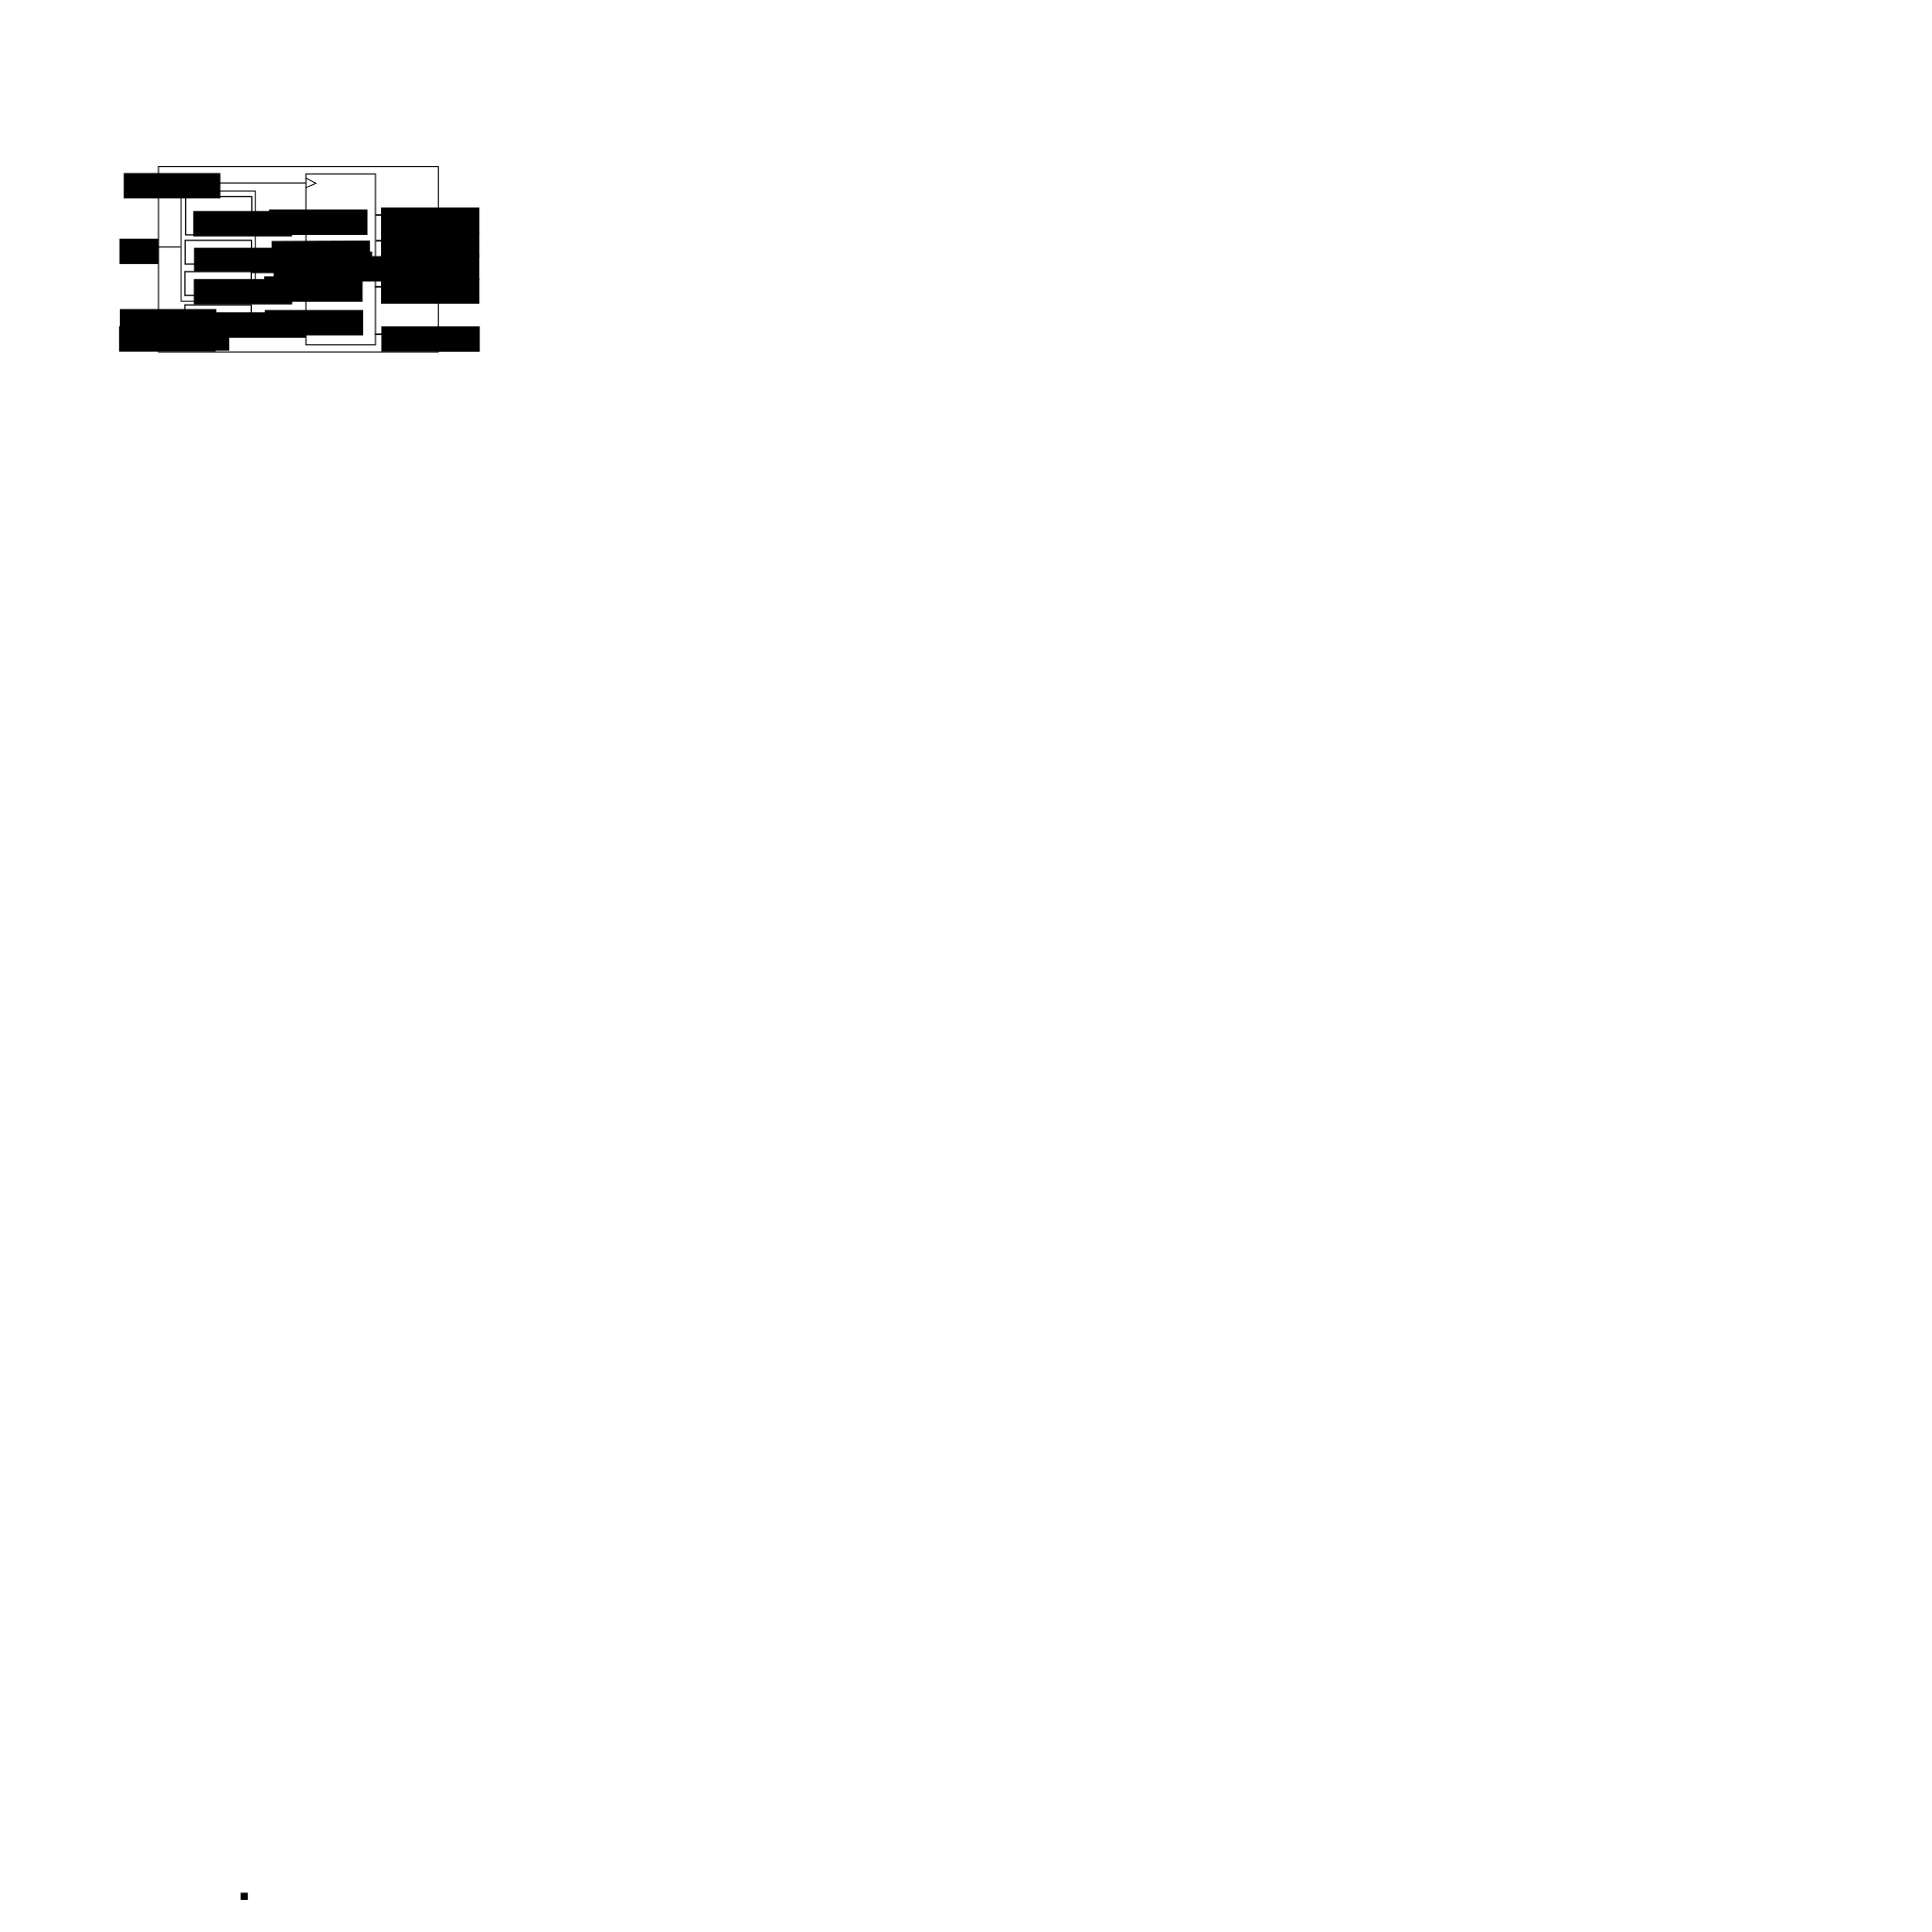
\includegraphics[width=\textwidth]{pict/patterngen.png}
\caption{Pattern Generator Core}
\label{fig:pattern_core}
\end{figure}

Figure \ref{fig:pattern_core} presents the \emph{Pattern Generator} IP core structure, input and output signals. Pattern Generator core consists of CCD Control FSM and control and status registers.  Pattern generator is responsible for generation of low-level clocking waveforms. It is fully programmable and can generate arbitrary waveforms, with resolution up to one clock cycle. CCD Control FSM is internally realised as FSM with stack. Microinstructions are kept in dual-ported BRAM memory - Pattern Generator behavior can be reconfigured by writing new set of instructions. The PS can program core control registers, status registers, and BRAM using an AXI Lite bus. Pattern Generator has configurable set of input and output lines - this is however non  software programmable (FPGA bitstream has to be reconfigured). If microprogrammed FSM with stack turns out insufficient it can be easily replaced with soft-core microcontroller such as \emph{picoBlaze}. Such microcontrollers have constant instruction fetching and execution time and better computational capabilities than FSM with stack, so can be seen as alternative. \\
The CCD Control FSM is currently configured to use following signals: 
\begin{itemize}
\item CLK – input clock,
\item BIN\_EN – chooses optional binning mode, 
\item RST – FSM reset, 
\item HW\_TRIG – hardware trigger, 
\item timer signals – counter that measures the exposure time,
\item CCD* - CCD control signals,
\item CNV0-3 – ADC conversion start signals
\item AUX SYNC – synchronization signals for other cores (e. g. Peltier cooling)
\item VIDEO SYNC – video synchronization signals for video DMA engine
\end{itemize}

Status register – reflects the current state of the Pattern Generator FSM.

\subsubsection{Trigger IP}
\begin{figure}[H]
\centering
\includegraphics[width=0.9\textwidth]{pict/trigger_ip.png}
\caption{Trigger IP Core}
\label{fig:trigger_core}
\end{figure}

\emph{Trigger IP} structure is shown on figure \ref{fig:trigger_core}. Trigger core accepts external arm, trigger, bld0\_action and bld1\_action signals. In order to use external shutter blade control signals, camera has to be put into appropriate state first \ref{sec:camctrl}. All hardware control signals are connected to the Global Interrupt Controller and are handled by appropriate RTOS interrupt handler functions which also provide timestamping. 


\subsection{CCD signal readout}
\label{sec:ccdreadout}
Figure \ref{fig:CCD_sections} presents block diagram of the internal structure of the E2V 23x--84 sensors. Andanta\footnote{According to current Andanta documentation} device is similar to E2V, but image area is divided in two sections instead of four. To avoid confusion, naming conventions for common elements in both sensors will be taken from E2V documentation. 

Sensor's image area is divided to sections with separate clocking signals which allow to move charge to two readout registers EF and GH. Both registers are connected to two output amplifiers: G and H to GH register, E and F to EF register. Charge from the readout register can be read from a single or both amplifiers. To allow such operation, registers have two clocking regions which divide it in the middle. 

\begin{figure}[ht!]
\centering
\includegraphics[width=0.5\textwidth]{pict/CCD_sections.png}
\caption{Block diagram of E2Vs' CCDs}
\label{fig:CCD_sections}
\end{figure}


Figure \ref{fig:CCD_IOs} shows the clocking regions of the sensor. Naming conventions is coherent with output amplifier and image region symbols. Each section belonging to common image half have separate clocking signals but same direction of clock indexing. Situation is similar with the horizontal register clocks. 

\begin{figure}[ht!]
\centering
\includegraphics[width=0.5\textwidth]{pict/CCD_IOs.png}
\caption{Clocking sections of the 23x-84 CCD sensor}
\label{fig:CCD_IOs}
\end{figure}

If whole half of the image will be transferred to the same horizontal register, a common clock for both sections can be used. Similar solution is possible for horizontal clocks. Such design allows to reduce number of FPGA pins, simplify HDL and analogue electronics design. Such solution allows to read-out the CCD in various way:
\begin{itemize}
\item Split full frame through four amplifiers,
\item Split full frame through two amplifiers,
\item Full frame through any single amplifier.
\end{itemize}

The limitation is that there will be no possibility to split frame in other way than in half. For example section D will always be read through the same horizontal register as section C. Situation is identical with sections A and B.

Output amplifier clocks can be shared by all outputs. If output is not used (i.e. charge is transferred only to one end of the horizontal register) it will still be clocked as an operating one. Such operation should not degrade performance and can simplify electronics design of the control buffers. Drawback of such solution is lack of possibility to clock the outputs independently, i.e. to speed up read--out outside of specific Regions Of Interest (ROI). Justification of taken approach is the fact that independent clocking has been discouraged by CCD manufacturers due to excessive noise caused by ground coupling.


Figure \ref{fig:CCD_Readout} presents schematic block diagram of the described system. CCD inputs and outputs have been divided by the functionality and phase i.e. vertical clock, phase 1 for section A is VP1-A. As described before, image area clocks drivers for section in the same half of the sensor are shared. In case of three--phase sensors such as Andanta's CCD4150A phase 4 of the horizontal clock will not be used.


CCD outputs are read by separate, independent AFE and ADC channels, which are described in detail in subsection \ref{sec:afe}.

\begin{figure}[H]
\centering
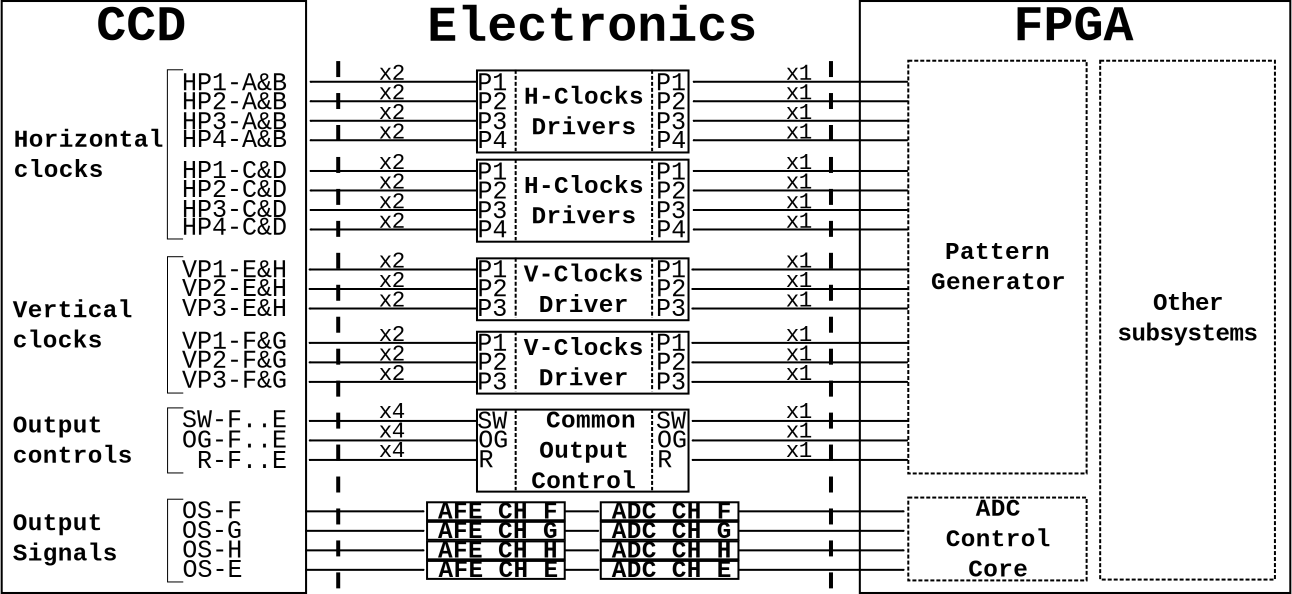
\includegraphics[width=\textwidth]{pict/CCD_Readout.png}
\caption{Schematic block diagram of CCD readout system}
\label{fig:CCD_Readout}
\end{figure}




\subsubsection{CCD readout windowing}
\label{sec:windowing}
Camera is able to increase read--out speed by entering windowing mode. Higher frame rate is accomplished by selection of specific ROIs in the image. Rest of the pixels are either dumped when shifted to horizontal register or clocked at higher read--out speed (with higher noise). Increase in frame rate depends on ROI area and shape. 

Due to adopted hardware architecture windowing is realised using exactly 4 fully symmetric readout windows as shown in the figure \ref{fig:windowing} - one in every CCD quadrant. Pattern Generator core is responsible for readout windowing control and synchronization.

\begin{figure}[ht!]
\centering
\includegraphics[width=0.7\textwidth]{pict/windowing.png}
\caption{}
\label{fig:windowing}
\end{figure}

Exemplary windowing mode readout time calculation is presented below. The simplest and the most useful case is considered - when 4 windows are all grouped together in the origin, making one bigger centred window as shown on \ref{fig:windowing2}. Calculations are based on \emph{E2V CCD model 231-84} technical data.

\begin{figure}[ht!]
\centering
\includegraphics[width=0.7\textwidth]{pict/windowing2.png}
\caption{}
\label{fig:windowing2}
\end{figure}

It is assumed that combined window is of  512x512 pixels size and that CCD is read out in 4 channel mode. \\

Line charge transfer time for dumped regions:
\begin{equation}
(4096-512)\cdot (65\mu s+17,5\mu s) \cdot 0,5=0,15s
\end{equation}


Line charge transfer for clocked regions:
\begin{equation}
0,5 \cdot 512 \cdot 65 \mu s=0,02s
\end{equation}


Clocking of ROI out of readout registers (using 2MHz clock):
\begin{equation}
(2048\cdot 500ns) \cdot 256=0,26s
\end{equation}

Total readout time:
\begin{equation}
0,15+0,02+0,26=0,43s
\end{equation}

For 512x512 pixel window the lowest achievable readout time is is 0,43s (2,3 fps). Actual frame rate will be even lower because of exposure, data handling and network transfer time. This compares with baseline full frame acquisition time of about 2,5 seconds.

\newpage
\subsubsection{Binning}
Camera hardware is capable of pixel charge binning independently in horizontal and vertical directions. For vertical binning, multiple rows can be summed in the horizontal register -- process is limited by the full well capacity of the register itself. Vertical binning happens at the output amplifier structure where multiple pixels can be summed at the output well. Again, limitation is full well capacity of the output node. Binning is achieved by feeding the CCD with specific clocking sequences, which are generated by Pattern Generator. 

\subsubsection{Antiblooming}

Blooming is phenomenon which occurs in the CCD devices when generated charge is greater than full well capacity. Overflowed charge is then "spilled" to the surrounding horizontal or/and vertical pixels. Effect occurs when bright light sources are present during sufficiently long exposure.

Antiblooming methods are designed to reduce the effect, by draining excess charge. Most common technique is to implement additional drain into the pixel structure. Due to the specific application of the Neostel Camera, hardware antiblooming may not be suitable because of its major drawback -- reduction of the fill factor.

Clocked Antiblooming (CAB) is another technique used to reduce blooming effects. It does not require special pixel structure and does not change fill factor. During integration period, clocking signals are applied to the CCD image area clock inputs in order to generate minority charges in the $Si-SiO_{2}$ interface. When overflow occurs, excessive electrons recombine with generated holes. Depending on the specific sensor, CAB can dissipate charge of size of dozen full well capacities.  

Among the main drawbacks of clocked antiblooming operation is the limitation of CCD dynamic
range over the limitation of pixel full well capacity (FWC). The FWC can be thought of consisting of 2
main components, a surface-FWC and a bulk (buried)-FWC. Under normal (non-CAB) operation, the
bulk-FWC will dominate the overall FWC, but under CAB-operation, the surface-FWC will mainly
contribute.
As a consequence, the overall-FWC of the CCD will be reduced under non-blooming environmental
conditions, although CAB is actually meant for increasing FWC, but only under blooming conditions.
A rough estimation example for the reduction of FWC under CAB – operation and nonblooming conditions is following:

\begin{itemize}
\item FWC normal value (normal non-CAB operation): e.g. 60.000 DN (= Digital Numbers)
\item FWC for CAB (CAB-operation, no blooming): e.g. ca. 55.000 – 58.000 DN
\end{itemize}


Another drawback of CAB is potential slew rate shifting under sub-optimal signal alignment
conditions; this adds noise over spurious charge induced, although this effect may be lower with our
4k x 4k-CCD in comparison to other devices, due to relatively low RC-time constant.

\subsection{AFE and CCD signal conditioning}

The main task of the Analogue Front End (AFE) is to adjust CCD output signal to the input of an ADC. Important factor that needs to be consider when design AFE is selection of the ADC. Resolution of the converter limits the systems performance because of the quantization noise. Another important factor is sampling rate which determinates number of samples per pixel and limits Digital Signal Processing capabilities of the system.

This section describes video signal path from the CCD output through AFE to the sampling process. As pointed out in section \ref{sec:ccdreadout}, selected sensors have four parallel outputs and each has independent signal processing channel. To simplify the documentation a single channel and processing is describe, but presented information are valid for all outputs.

According to ANDANTA, CAB should provide 100x reduction in blooming for integration periods of sixty seconds.

\subsubsection{Analogue to Digital Converters}

System performance is limited by all source of the noise. One of them is the ADC itself, as it introduces quantization noise to the sampled signal. The SNR of the ADC resulting from the finite resolution of the converter is equal to \ref{eq:qnoise} \cite{mt-001}.

\begin{equation}
\label{eq:qnoise}
SNR = 6.02 \cdot ENOB[dB] + 1.76dB + PG
\end{equation}

Where ENOB stands for number of significant bits and PG is Process Gain which will be described further in this section. Table \ref{tab:qnoisetab} presents relation between quantization SNR and ENOB.

\begin{table}[ht!]
\centering
\caption{CCD comparison}
\label{tab:qnoisetab}
\begin{tabular}{c|c}
ENOB & SNR[dB] \\ \hline 
14 & 86 \\ \hline 
15 & 92 \\ \hline 
16 & 98 \\ \hline 
17 & 104 \\ \hline 
18 & 110 \\ 
\end{tabular}
\end{table}

To accomplish high SNR, over 100dB a high resolution ADC is required. At the same time fast sampling rate is desired -- minimum twice the pixel clock to sample both pixel and reference level. ADC technology comparison shows that high resolution ADC such as Sigma--Delta converters have insufficient sampling rate. On the other hand, flash ADCs used i.e. to build sampling oscilloscopes have resolution of 8-10 bits. 

Only technology which is close to requirements is Successive Approximation ADCs (SARs). Camera is using AD7960 converters which have 18 bits resolution with 5Msps. The sampling rate is more than two times faster than sampling clock, which gives two samples per pixel. 

For digital signal processing more samples are needed, i.e. to perform digital filtering. To achieve higher sampling rate, four parallel ADC has been connected to each AFE channel. Combined frequency of the system is 20MHz, which gives eight samples per pixel (four on each level). Such solution causes issues related to parameter differences between the four ADCs -- such as linearity characteristics. Fortunately effects of these parameters for SAR ADCs are limited to two least significant bits. Dropping the bits from the video signal will solve the problem of parameter differences.

Using smaller number of bits decreases the quantization related SNR. It can be however increased by signal processing by digital filtering. It would be perform anyway to reduce bandwidth and attune noise introduced by analogue devices in processing chain. Process Gain (PG) in equation \ref{eq:qnoise} can be described by \ref{eq:progresg} \cite{mt-001}.

\begin{equation}
\label{eq:progresg}
PG = 10 \cdot \log_{10}\frac{f_{s}}{2 \cdot BW} [dB]
\end{equation}

Where BW represents limitation of bandwidth introduced by the filtering and $f_{s}$ is sampling frequency. If simplest filtering is used -- i.e. averaging by n, filter has coefficients equal to $\frac{1}{n}$ and bandwidth equal to $\frac{f_{s}}{2n}$. Gain due to filtering can be described by \ref{eq:progrq1} \cite{mt-001}.

\begin{equation}
\label{eq:progrq1}
PG = 10 \cdot \log_{10}\frac{f_{s}}{2\cdot\frac{f_{s}}{2n}} = 10\cdot\log_{10}(n)[dB]
\end{equation}

For oversampling by 8 PG is equal to 9 dB. Hence system quantization SNR is equal to 107 dB and can be increase by further reduction of digital filter bandwidth.

\subsubsection{Available Sampling Schemes}

Each pixel is sampled with 18-bit resolution and in basic acquisition mode consists of two samples: one of video level and another of black level. The Readout frequency is programmable and can be switched between 2MHz and 500kHz. In case of oversampling number of samples of both video and black level is multiplied by oversampling factor. In case of 4x oversampling both video and black level have 4 samples each.  Each group of ADCs is triggered by same sequence of triggering signals: CNV0, CNV1, CNV2 and CNV3. Separating these signals in phase allows for oversampling. Repeating the sequence enables more than 2x oversampling factor. Repeating sequence twice allows for 4x oversampling as shown on figure \ref{fig:sampling_4x}. Repeating sequence 8 times enables 16x oversampling as shown on figure \ref{fig:sampling_16x}. Figures below show both 4x and 16x oversampling modes, taking into consideration relative timing dependencies, CCD signal phases and pixel clock period. \\ 
For example in 4x scenario - clock period is 500 ns, reset pulse is 100 ns, while both black and video level are about 200 ns each. As shown on figure, 5MSPS (200ns) conversion time limit is observed for every ADC.

\begin{figure}[H]
\centering
\includegraphics[width=\textwidth]{pict/CCD_sampling_4x.png}
\caption{CCD sampling method for each of CCD readout channels in 4x oversampling mode (one channel shown) 2 MHz pixel clock}
\label{fig:sampling_4x}
\end{figure}

\begin{figure}[H]
\centering
\includegraphics[width=\textwidth]{pict/CCD_sampling_16x.png}
\caption{CCD sampling method for each of CCD readout channels in 16x oversampling mode (one channel shown) 500 KHz pixel clock}
\label{fig:sampling_16x}
\end{figure}

\subsubsection{Jitter}
All signals sourced in the FPGA (clocks and data signals) are characterized by a certain amount of jitter (even 1ns pp). For some signals, the jitter is noncritical, provided that adequate timing margins are ensured. For the ADC conversion trigger, jitter is a critical parameter for achieving the expected SNR. Internal Input Output Blocks in the FPGA will resynchronize CNV signals coming from the CCD Driver. 
The entire readout electronics has a common clock source. All clocks responsible for the CCD readout, sampling, and charge shift are derived from a common clock source. These clocks have different frequency but remain in constant phase relationship.

\subsubsection{Analog Signal Path}

The block diagram below \ref{fig:analog} shows the signal path between a single CCD output and four ADCs designated for each channel. 
%grafika mi się wyświetla jako czarna Piotr Zdunek
\begin{figure}[H]
\centering
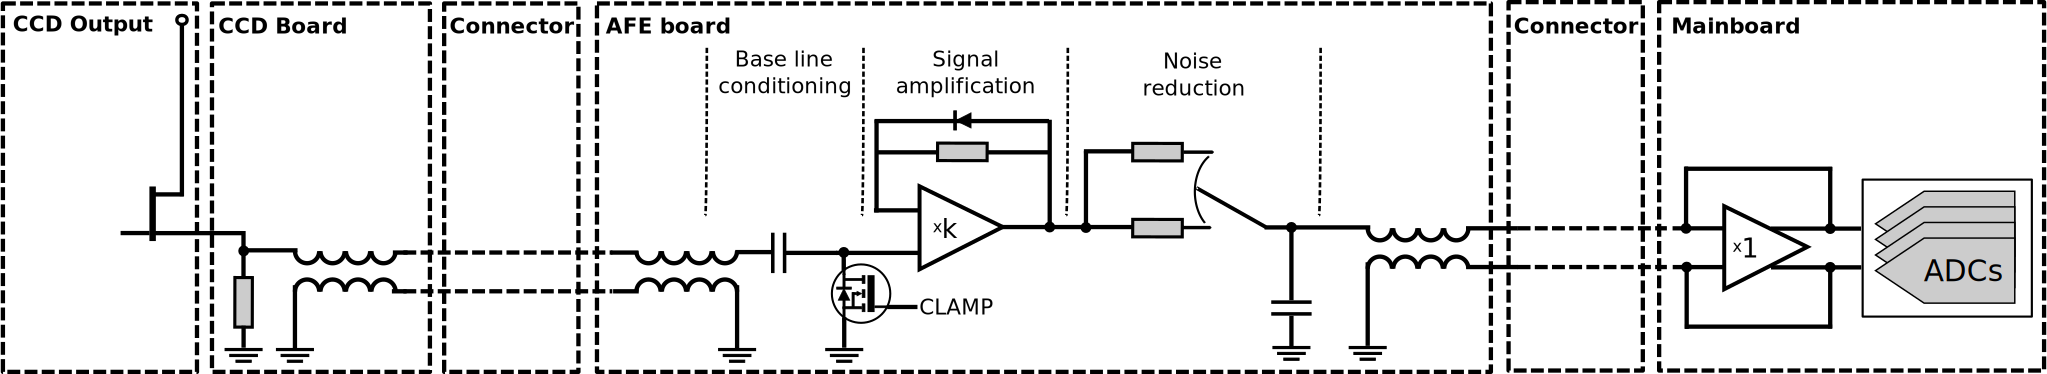
\includegraphics[width=\textwidth]{pict/afe_schem.png}
\caption{Analogue signal path}
\label{fig:analog}
\end{figure}

The output of the CCD is an open drain configuration transistor. To be operational, it needs an additional resistor load, which is installed on the CCD board. To lower noise induced by external sources baluns are used and signal is transmitted through a differential line. On AFE board, a capacitor is placed to cut off the DC level from the CCD that tends to depend on temperature and additional factors. A MOSFET transistor driven by a CLAMP signal is used to shift the reference level to zero volt. This solution ensures that the pixel level voltage will be negative and referenced to the ground. The reset pulse will be therefore positive, and has to be cut out to protect the signal amplifier input from overvoltage. The protection is implemented by a diode in operational amplifier's feedback loop. \\

The noise reduction subsection is implemented as a RC low-pass filter with an adjustable bandwidth. Switching the serial resistance of the filter changes the pass frequency. A small resistor is used to provide the wide bandwidth required to transfer sharp signal edges. When the reference or pixel level is reached, the DC value of the signal is measured. To minimize noise, the filter is switched to higher resistance that narrows the bandwidth. The noise added by the filter depends only on the capacitor value. 
After noise reduction, the signal is transformed from a single ended to a differential signal with a high common mode rejection of RF noise. The signal is adjusted on the Mainboard to fit input levels accepted by the ADC.
For the initial simulation in a Tina-TI simulator, an equivalent circuit has been designed. The signal amplification was implemented with an OPA355 OPAMP, whereas the buffering was realized with a THS4531 OPAMP. The results of this filtering are presented on figure \ref{fig:noise}. SNR was simulated with respect to the full scale ADC input. Results present amount of noise introduced by AFE and does not include CCD noise. Nonetheless the bandwidth switch can increase AFE's SNR up to tens of decibels for low frequencies. 

Figure \ref{fig:bwswsim} presents results of the filter in time domain. Additional noise signal has been generated with use of SciLab and feed as periodic signal at the input of the AFE channel. Another voltage source is simulationg pixel readout from the CCD. As can be seen, when the bandwidth switch is used, noise level is noticeable reduced.

\begin{figure}[H]
\centering
\includegraphics[width=\textwidth]{pict/snrsim.png}
\caption{Filtering results in frequency domain}
\label{fig:noise}
\end{figure}


\begin{figure}[H]
\centering
\includegraphics[width=\textwidth]{pict/bwswsim.png}
\caption{Filtering results in time domain}
\label{fig:bwswsim}
\end{figure}

The AFE is placed on a dedicated, shielded module. Common mode chokes and Signal Integrity control methods are used to minimize cross talks.


\subsection{Digitized CCD pixel data processing flow}

\begin{figure}[H]
\centering
\includegraphics[width=0.8\textwidth]{pict/pixel_proc.png}
\caption{CCD pixel processing flow}
\label{fig:pproc}
\end{figure}

\subsubsection{Overview}
ADC interface processing data flow is shown on figure \ref{fig:pproc}. Firstly conditioned CCD signal is sampled and digitized by 16 ADCs (in case of 4 channel readout with oversampling) and read into FPGA by 16 ADC readout cores. After that, samples are collected in buffer waiting for processing - buffer length is dependent on oversampling ratio - 8 samples for 4x and 32 samples for 16x (half of them video level and another half - black level). Samples collected in buffer are then processed giving in result one 16-bit pixel value. Finally pixels are sent along video synchronization signals to the DMA subsystem. \\
Nominal size of CCD sensor is 4096x4096 pixels . Taking into account oversampling 4x and 16x, raw frame sizes are respectively 256MB and 1024MB. In order to speed up processing and save memory, samples are processed and decimated on the fly in FPGA as described in DSP subsection \ref{sec:dsp}. After processing each pixel has 16-bits. Resulting image frame written to memory has size of 4096x4096x2 = 32MB. 

The ADC Interface consists of ADC readout cores - 4 for each channel, samples buffer and DSP block. ADC interface uses signals generated by Pattern Generator for synchronization. Pixel data and video synchronization signals are connected to the DMA engine, as described in the next subsection. Detailed description of all processing blocks is given below.

\subsubsection{ADC readout core}
Each ADC readout core is responsible for generating the readout clock for the ADC, readout and deserialization of ADC data. The core is also responsible along with Pattern Generator for keeping control signals for ADC within timing limits. Each core consists of control FSM, timing counters, clock gating primitive, shift register, IO buffers and programmable delay element needed by clockless ADC readout mode.

\subsubsection{Sample buffer}
Role of sample buffer is to gather all samples (both black and video level) belonging to single CCD pixel for further processing. It can be realised as a multiplexer and set of registers. 

%TODO MJ
\subsubsection{Digital Signal Processing Core}
\label{sec:dsp}

Digital Signal processing is aimed to increase image quality. Few techniques are being considered and will be tested during prototyping period. The CCD signal resembles discreet signal and DC states are measured. Estimation techniques can be used to find and remove low frequency noise observable as patterns. After the estimation low--pass digital filtering will be applied to enhance SNR and attune some portion of higher frequency noise introduced by AFE and external sources. Final step of the processing is digital Correlated Double Sampling (CDS). It will attune low frequencies (such as flicker noise) and remove correlated reset noise and reference level from the signal. 

\begin{figure}[H]
\centering
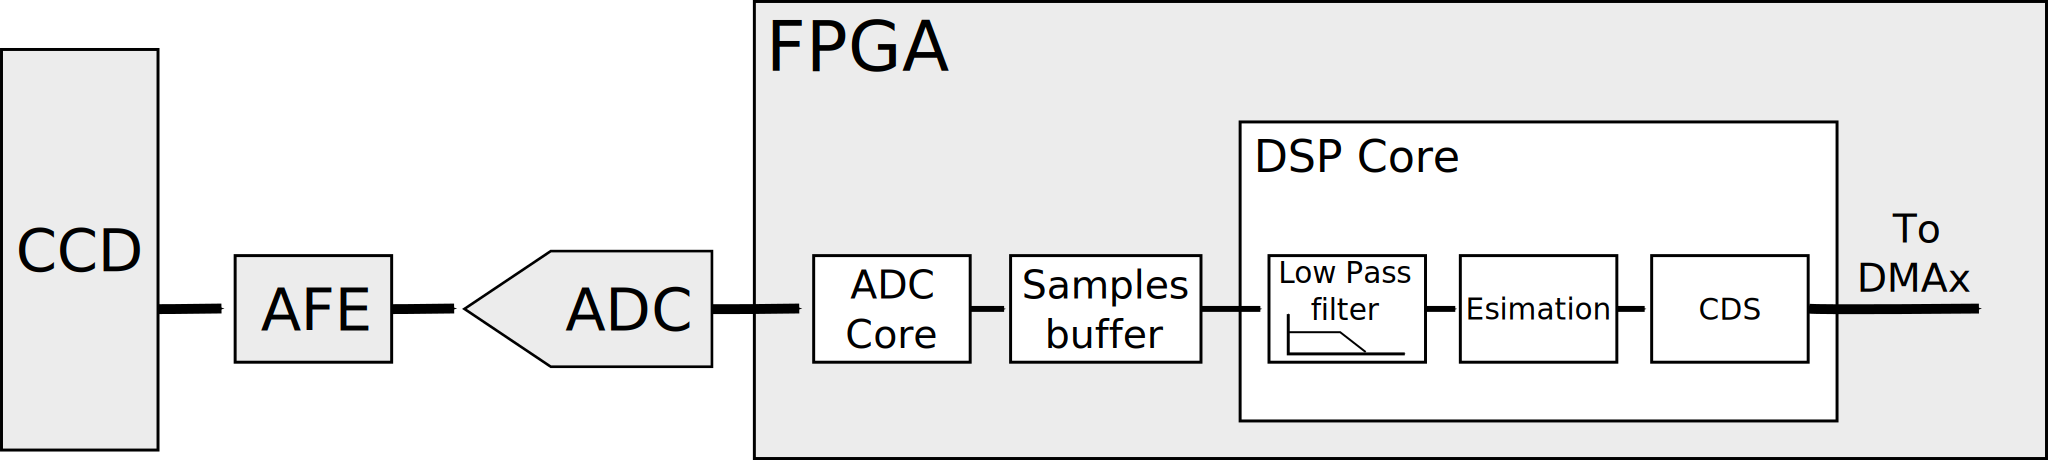
\includegraphics[width=\textwidth]{pict/dspcore.png}
\caption{DSP core internal structure }
\label{fig:dspcore}
\end{figure}


\subsection{DMA data flow}

\subsubsection{Overview}

\begin{figure}[H]
\centering
\includegraphics[width=0.8\textwidth]{pict/przeplyw_danych.png}
\caption{Video data flow}
\label{fig:video_flow}
\end{figure}

To leverage the ZynQ SoC design philosophy, camera data acquisition module is based on existing Intellectual Property (IP) cores provided by Xilinx along with Zynq design tools. Xilinx provides IP modules compatible with the AXI bus specifications, designed to fulfill common tasks such as handling DRAM memory transfers. \\
Digitized and processed CCD video pixel data flow is shown on figure \ref{fig:video_flow}. The ADC Interface outputs four channels of parallel video data , each conforming to one read channel. During normal readout each ADC interface channel outputs 2048x2048x2=8MB of data. Enabling binning or less than 4-channel readout changes this value, and DMA engine needs to be programmed accordingly. Parallel video data is converted by VID IN TO AXI4 STREAM core into AXI stream packets, which are then fed to the DMA engine, and written to system DDR memory - each channel into separate base address. Written image data is contained in one continuous memory block but due to CCD readout method, order of image pixels in memory is different than physical one in CCD matrix. To obtain the final picture, an additional software pixel reordering is required. \\
The Camera DMA engine utilizes following Xilinx IP cores:

\begin{description}

\item \textbf{AXI DMA} \hfill \\
The AXI DMA v 7.1 is a general purpose DMA controller which can handle video data as well. It is programmable and supports various DMA schemes. The DMA core is fully duplex – supports both read and write channels to the memory – in this case only write channels are used. The DMA transfers data over the AXI Stream Bus (address-less data packets) and outputs data using the AXI Memory Mapped Bus (data packets with addresses).
\item \textbf{VIN2AXIS} \hfill \\
The Video In To AXI Stream v 3.0. 2 AXIS core provides the interface between clocked, parallel video data and the AXI Stream bus. Internally it is built around dual ported FIFO that acts as a bridge between two asynchronous clock domains – video data pixel clock and AXI Stream bus clock. FIFO acts also as a data buffer and its depth is programmable.
\item \textbf{AXI Interconnect} \hfill \\
AXI Interconnect v 2.1 acts as a bridge between AXI MM cores and hardware memory interconnect. It is capable of translating the AXI protocol version (IP cores use version 4, while interconnect hardware uses version 3) and the arbitration between connected AXI MM endpoints.

\end{description}

\subsubsection{Clocking}
Neostel Camera digital interface is clocked from two asynchronous clock sources. DMA and AXI subsystems are clocked from IO PLL, which is connected to Zynq 33.33MHz clock generator. Pattern generator and ADC interface clock is derived from stable external Programmable Clock Generator. Both clocks have frequency of 100MHz.

%TODO   vii) "assembly" of pix values into image and data flow of image
\subsection{Software image assembly}

\todo[inline, caption={FITS}]{Paweł, proces zapisu zdjęcia do FITSa trzeba opisać, ESA to chciała: vii) "assembly" of pix values into image and data flow of image /MB}

\subsubsection{FITS}

It was verified that FITS meets the specification regarding the required header size for time stamping. The FITS format is very versatile since it allows the storage of several non-typical parameters in its header. It is useful for the foreseen monitoring of e.g. temperature and humidity inside and outside the chamber, vibration level, critical digital voltages and currents, TEC current, CCD voltages, and operational status (exposure, readout, idle, failure, vacuum, etc.).
The file format will be implemented according to the FITS 3.0 standard defined in the  “Definition of the Flexible Image Transport System (FITS)” document from the FITS Working Group published on 18 November 2010.
The output of the camera with diagnostic data will be fitted into a Single Image FITS (SIF) since the additional diagnostics and time-stamping information can be stored as header keyword values in standard printable ASCII (positions 32-126 in the ASCII table) strings, which limitation far exceeds the need of representation diagnostic values and timestamps. Minor data can be stored as comments if necessary.
The FITS standard allows storing image data in form of a two-dimensional matrix with integer values. The integer size can be defined within an up to 64-bit representation that exceeds the 16-bit readout of the ADC data. Since there is no limitation for the file length, additional data can be added if necessary.
A CFITSIO/CCFITS library will perform the storage of the FITS file. The FITS headers and HDUs will be filled following the NEO-CAM-DR-0150 requirement. Test images (with filled headers and stub raw data) will be supplied with camera.

\subsection{Camera control}
\label{sec:camctrl}

\subsubsection{Overview}

\begin{figure}[H]
\centering
\includegraphics[width=\textwidth]{pict_ipc/oses-control.png}
\caption{Neostel camera control}
\label{fig:oses_ctrl}
\end{figure}

The camera is running two operating systems: an embedded Linux system and RTOS. Linux is used for the communication and the high level control of the entire system. RTOS is used for low level control and time critical tasks. The SoC that is used in this design is a two-core unit that supports AMP operation. This way one core is used for Linux and the other is reserved for RTOS. \\
Calibration activities: the flat fielding, dark current, bias subtraction and pointing model update will be handled by software, but can also be implemented directly into the camera firmware, if necessary.

\subsubsection{RTOS}
The purpose of using a Real Time OS is to provide direct control over all camera subsystems. RTOS is capable handling of hardware related events and processes in deterministic time. The RTOS running APU core is connected through an AXI Lite bus with FPGA - implemented IP cores. \\
Main IP-cores directly controlled by RTOS:

\begin{itemize}
\item Pattern Generator
\item ADC Interface
\item Shutter interface control
\item Cooling subsystem
\item Minor peripheral control (sensors etc.)
\end{itemize}

IP cores have control, configuration, and status registers when applicable. In accordance to the adopted architecture, there is no direct access from network to the RTOS. All remote network interactions are handled by Linux OS, to which RTOS is connected with an IPC subsystem. IPC uses shared memory which includes built-in OCM inside the Zynq SoC. IPC subsystem provides basic IPC mechanisms such as spinlocks and message queues. Apart from beforementioned features, main camera command process is also running on RTOS. 

\subsubsection{LINUX OS}
To provide the remote control and data acquisition of the camera, Linux OS is used. It provides a flexible, convenient method to achieve:
\begin{itemize}
\item Facility level integration with other equipment using an EPICS SCADA server
\item Data encapsulation in self-describing, interchangeable format using FITS file format
\item API for camera functions described in this document
\item Data storage on external machines using transports based on TCP/IP, e.g. NFS or FTP
\item Easy camera access with Linux tools, such as SSH etc.
\item Internal diagnostic processes checking for software and hardware faults (including external hardware watchdog for system hung).
\end{itemize}

Linux OS is based on Yocto embedded Linux build system. Linux is compiled from BSP and customized to fulfill the requirements of the camera. There are several processes running continuously.

\subsubsection{Low level control signals}

\todo[inline, caption={Dodać potwierdzenie gotowości}]{Trzeba opisać że po ARM zostanie wysłanie potwierdzenie gotowości po EPICSie i dopiero wtedy TRIGGER bedzie aktywny. /KZ}

\todo[inline, caption={Feedback wykonania akcji przez shuttera w trybie diagnostycznym}]{Trzeba przemyśleć jak (najprawdopodobniej EPICS) dać feedback że shutter wykonał ruch w trybie diagnostycznym, czyli sterowania zewnętrznego migawką. /KZ}

\todo[inline, caption={Zdefiniować sygnały i opisać warstwę fizyczną transoptorów}]{Trzeba tu opisać co jest dostępne ze zewnątrz kamery i jak to wysterować oraz zdefiniować jak mają wyglądać sygnały. Ustalone zostało że reagujemy na zobaczę a sygnał ma trwać conajmniej 10us /KZ}

Main camera control signals (ARM, TRIGGER, BLD0\_ACTION, BLD1\_ACTION) are realised as hardware lines to unify and simplify control logic. Additional control such as configuration, diagnostics, logging etc. is implemented using software IPC mechanism between operating systems. For description of IPC subsystem refer to chapter \ref{chap:ipc}.

\begin{figure}[H]
\centering
\includegraphics[width=0.7\textwidth]{pict/cam_command.png}
\caption{Camera control signals routing}
\label{fig:camcmd}
\end{figure}

Figure \ref{fig:camcmd} presents hardware control signals routing between various camera subsystems. Control signals are all routed through \emph{Trigger IP}, which selects which signals pass through, depending on the state of the camera. For example external \emph{bld0\_action} and \emph{bld1\_action} signals are enabled only in diagnostic camera mode.

\begin{description}
\item \textbf{ARM} \hfill \\
Arming camera is required before each image registration. ARM signal is connected to the interrupt serviced on APU Core running RTOS. Arming camera is a software process in which various camera subsystems including DMA, ADC Interface, Pattern Generator, Trigger IP etc. are programmed according to configuration stored in configuration buffer. Shutter is reset and trigger is then armed and whole system is prepared for single or series image registration.

\item \textbf{TRIG} \hfill \\
Trigger signal starts process of image acquisition in normal mode, and starts exposure and readout process in diagnostic mode. In both cases trigger is realised in hardware (Pattern Generator) to minimise delay and jitter.
\item \textbf{BLD0\_ACTION} \hfill \\
Shutter blade0 open/close signal.

\item \textbf{BLD1\_ACTION} \hfill \\
Shutter blade1 open/close signal.

\end{description}

\subsubsection{RTOS camera control task states}
\label{sec:control_fsm}

\todo[inline, caption={Zamiec blade error na blade confirm}]{Uzgodnione zostało że migawka zamiast sygnału błędu wysyłać będzie potwierdzenie które będzie resetowane przez RS485. Na poziomie kamery będzie licznik do timeoutu w razie gdyby migawka nie wysłała potwierdzenia. /KZ}

Figures \ref{fig:camstate}, \ref{fig:camstatediag} and \ref{fig:camstatetesting} present camera control FSM. After camera start-up, all systems are initialized and camera goes into \emph{idle} state. Idle state is the default standby state - in this mode camera waits for commands - can be armed, switched into diagnostic mode or camera subsystems can be tested. In case of error occurring during operation, camera goes into \emph{error} state and camera firmware (RTOS) has to be reset (reloaded).

\begin{figure}[H]
\centering
\includegraphics[width=0.7\textwidth]{pict_ipc/camera_command.png}
\caption{Camera state diagram}
\label{fig:camstate}
\end{figure}

Diagnostic mode is separate state subtree which enables independent shutter control in diagnostic and calibration purposes - in normal mode shutter is operated by Pattern Generator and cannot be operated manually \ref{sec:shutctrl}.

\begin{figure}[H]
\centering
\includegraphics[width=0.4\textwidth]{pict_ipc/diagnostic_mode.png}
\caption{Diagnostic mode state diagram}
\label{fig:camstatediag}
\end{figure}

Camera subsystem self-test can only be carried out in idle mode.

\begin{figure}[H]
\centering
\includegraphics[width=0.5\textwidth]{pict_ipc/testing_mode.png}
\caption{Submodules testing state diagram}
\label{fig:camstatetesting}
\end{figure}
 
\subsubsection{Triggering}
Multiple NEOSTEL camera image captures can be triggered in two scenarios: by hardware and by software. An external hardware trigger is applied through opto-coupled logic level inputs, mitigating ground loop problems. An external electronic module can control analog trigger signals for all cameras. The cameras themself can control the image capture triggering via EPICS as well. A centralized external trigger will ensure the synchronization between individual cameras and will coordinate the functionalities of the different cameras in order to keep them in temporal coincidence. Each control signal assertion is time-stamped. Trigger signals are: arm camera and trigger. Shutter blades are controlled separately with signals: Open/Close blade \#1, Open/Close blade \#2 and can be controlled manually only when camera is in diagnostic mode.  The triggering scheme is depicted in \ref{fig:triggering}.

\begin{figure}[H]
\centering
\includegraphics[width=0.9\textwidth]{pict/triggering.png}
\caption{Neostel camera triggering scheme}
\label{fig:triggering}
\end{figure}
 
\subsection{Shutter control}
\label{sec:shutctrl}
%TODO
%Przemyśleć w jaki sposób ma trafiać sprzężenie zwrotne do linuksa, gdy kamera jest sterowana zewnętrznymi sygnałami sprzętowymi

RTOS camera control task operates in two distinct modes: \emph{normal mode} and \emph{diagnostic mode}. In diagnostic mode shutter control is completely independent of CCD readout, to allow for various testing procedures. Futhermore both shutter blades are independent from each other as well. There is no option for auto exposure in this mode. In normal mode shutter blades are operated in unison and there is no possibility of operating them separately.

\subsubsection{Diagnostic mode}
As stated before, in diagnostic mode shutter control is completely independent of CCD readout and shutter modules are independent of each other, to allow for various testing procedures. In this mode shutter blades can be controlled manually only using external signals BLD0\_ACTION and BLD1\_ACTION.
\subsubsection{Normal mode}

In normal mode shutter blades are coupled together and are operated simultaneously. A precise time synchronization of the readout and shutter operation is ensured by readout and shutter controllers that are implemented entirely in hardware, in particular to avoid image smearing, e.g. by starting the read-out before a complete closing of the shutter.

\begin{description}

\item \textbf{Auto exposure} \hfill \\

\begin{figure}[H]
\centering
\includegraphics[width=\textwidth]{pict_ipc/shut_ctrl_auto.png}
\caption{Auto exposure Pattern Generator shutter control chart}
\label{fig:shutctrlauto}
\end{figure}

In auto exposure mode shutter is controlled by Pattern Generator - PG opens and closes shutter according to internal exposure timer. Trigger is used to initiate picture taking sequence including shutter operation \ref{fig:shutctrlauto}. Shutter control program checks for errors and communicates with shutter using direct control lines  and control lines through Zynq Core running RTOS. Time deadlines are provided for shutter operation - if operation completion is not confirmed on time, shutter control programs goes into error state.

\item \textbf{Manual exposure} \hfill \\
In manual exposure mode, shutter opening and closing is controlled by external signal. In this mode TRIG signal is used as both shutter opening and shutter closing signal. External control of BLD0\_ACTION and BLD1\_ACTION signals is disabled. Similarly as in automatic case, shutter operation checks are performed and errors are generated accordingly.

\begin{figure}[H]
\centering
\includegraphics[width=\textwidth]{pict_ipc/shut_ctrl_man.png}
\caption{Manual exposure Pattern Generator camera control chart}
\label{fig:shutctrlman}
\end{figure}

\end{description}

\subsubsection{Error handling}
According to adopted shutter architecture in case of either of shutter modules encountering problems during operation, appropriate error lines are asserted. These lines are connected to the GIC inputs. ISRs for shutter error lines are serviced under RTOS. In such case, RTOS polls shutter for error details through RS-485 interface and sends error event message to Linux through IPC mechanism.


%\subsection{Binning and windowing capability}
%Both binning and windowing capabilities are dependent on Pattern Generator program, and should be possible to realise without major changes in proposed camera architecture. It is then proposed to implement these features at later prototype stages.

\subsubsection{Boot sequence}
\todo[inline, caption={Boot sequence update}]{Stary boot sequence, przydałaby się dyskusja? Sporo się chyba zmieniło w kwestii diag./PZi}
When the input power is applied to the camera, the system starts booting. The Initial boot sequence works as depicted in the diagram below \ref{fig:bootseq}.
The boot sequence incorporates an initial system test. Basic peripherals needed for the operation are checked. Due to the fact that the system is a multi-camera design, the operational system image is stored remotely (e.g. on a server available via NFS). 
Initially, a test version is booted from the QSPI Flash memory. If the initial test has passed, the remotely available image is loaded and the system is restarted. In the second scenario a fail-safe system version is booted. 
The initial testing will be performed using Uboot procedures. The entire diagnostic output during the boot is logged on a SD card that is attached to the designed board to enable future problem tracing and debug possibilities.

\begin{figure}[H]
\centering
\includegraphics[width=1.0\textwidth]{pict/bootseq.png}
\caption{Boot sequence}
\label{fig:bootseq}
\end{figure}

\subsubsection{Overall control of exposure sequence}
This subsection presents exemplary description of camera operation during startup and single image frame acquisition. Low level camera control is based on FSM described in previous subsection \ref{sec:control_fsm}.

\begin{description}

\item \textbf{Camera initalization}
\begin{enumerate}
\item camera reset
\item system boot
	\begin{itemize}
		\item load system image to memory
		\item load linux
	\end{itemize}
\item software init
	\begin{itemize}
		\item lanuch linux camera software processes, i.e. camera control, logging, EPICS
		\item load and launch RTOS firmware
		\item camera control FSM goes into \emph{INIT} state
	\end{itemize}
\end{enumerate}

\item \textbf{Camera INIT state}
\begin{enumerate}
	\item load default configuration
	\item init camera submodules
	\item go to the \emph{IDLE} state
\end{enumerate}

\item \textbf{Camera IDLE state}
\begin{enumerate}
\item waiting for commands
\item if arm command received
\begin{itemize}
\item send arm\_acq event
\item program VDMAs
\item program ADC interface
\item program shutter control multiplexer
\item program Pattern Generator
\item program trigger core
\end{itemize}

\end{enumerate}
\item \textbf{Camera ARMED state}
\begin{enumerate}
\item wait for trigger
\item if trigger received 
\begin{itemize}
\item Pattern Generator is triggered
\item send trig\_acq event
\item go to the \emph{TRIGGERED} state
\end{itemize}
\end{enumerate}
\item \textbf{Camera TRIGGERED state}
\begin{enumerate}
	\item image registration
	\begin{itemize}
	\item Pattern Generator generates control signals for shutter, ADCs and VDMA subsystem
		\begin{itemize}
			\item shutter opening
			\item exposure
			\item shutter closing
			\item CCD readout and DMA transfer
		\end{itemize}
	\end{itemize}
\item send \emph{picture\_ready} event
\item go to the \emph{IDLE} state
\end{enumerate}

\item \textbf{Registered image software processing}
\begin{itemize}
\item linux process receives \emph{picture\_ready} event
\item linux process reads out frame data strucuture
\item shutter timing is recalculated from timestamps
\item FITS image is formed
\item FITS is sent by epics
\end{itemize}

\end{description}


\section{Linux - FreeRTOS IPC}
\label{chap:ipc}


%TODO
%PDR opisywany behawioralnie, nie wdawać się w szczegóły - pominąć dokładny opis struktur danych.
%Do obsługi dużych klatek (nadpróbkowanie 16x) należy przeprogramować zarówno VDMA jak i ADC interface. Trzeba podzielić dużą klatkę na mniejsze bo inaczej nie zmieści się w VDMA.

%Określić sposób ładowania systemów operacyjnych oraz sposób uruchamiania programów - w jaki sposób obejść problem z uruchamianiem cachu
%Dopracyzować poszczególne stuktury danych, aby można było oszacować ile cała impreza zajmie pamięci
%Doprecyzować listę i sposób kodowania rozkazów
%Doprecyzować listę, sposób kodowana i ew. rodzaj generowanych odpowiedzi
%Dokończyć mapę pamięci
%W jaki sposób ma być zrealizowana obsługa błędów na poziomie FreeRTOSa?
%Czy opisy sposobu testowania umieścić w oddzielnych dokumentach dotyczący poszczególnych modułów kamery?
%Jakie powinny być długości danych (np. timestampy? - 64 bit?) Timestamp: 32bit - sekundy 32bit- nanosekundy
%Opracować z Konradem specyfikację danych dla migawki
%Opracować strukturę danych dla peltiera
%Wyzwalanie triggera odbywać się będzie na linuksie


%TODO
%PYTANIA I PROBLEMY
% - Jest problem z DMA dla nadpróbkowania 16x - kontroler nie obsługuje tak dużych ramek obrazu (rozmiar podaje się w bajtach)
% - Jak zrealizujemy oknowanie sygnału z CCD?

%Do Pawła
% - Jak będzie wyglądał interfejs pomiędzy Epic a serwerem sterującym kamerą?
% - Czy diagnostyka będzie przeprowadzana przez Epica?
% - Ja robię diagnostykę na FreeRTOSie, Paweł na linuksie

\subsection{Introduction}

%\todo[inline, caption={IPC Polling/Interrupt}]{Czy podjęta została ostateczna decyzja odnośnie implementacji IPC na pollingu a nie przerwaniach? Można wykorzystać jedno przerwanie z GICa i jechać na nim, może to być lepsze rozwiązanie, na początku tylko więcej zachodu. Można sprawdzić to: http://henryomd.blogspot.com/2015/02/zynq-inter-process-interrupts.html  /PZi}

This section describes proposed interprocessor communication architecture to be used in Neostel camera. As it was decided beforehand that camera APU will operate in AMP mode running two independent operating systems - Linux and FreeRTOS, current section limits it's scope to those OSes and ARM Cortex A9 dual core architecture (Zynq - 7000). \\
System utilizes bidirectional communication based on message queues. Communication occurs between process running on one APU core and task running on the other. Process running on Linux OS issues commands, while FreeRTOS task reads and executes commands. For every command issued by the master there is one acknowledgement response generated by the slave. Commands are issued and executed sequentially, one at a time. Before next command can be issued, previous has to finish. Additionally FreeRTOS can send asynchronous event messages such as unexpected error to Linux, without being polled first. Both commands and responses are sent through their respective FIFO message queues implemented in shared memory regions.

\vspace{\baselineskip}
Key assumptions:
\begin{itemize}
\item asynchronous communication based on polling - no interprocessor interrupts (no need to write specialized linux driver)
\item master - slave architecture
\item commands, responses and data separation - commands and responses in FIFOs, data in their respective shared memory regions
\item sequential commands execution - one command at time
\item every command generates response
\item slave can send asynchronous event messages to the master
\item address table known at compilation time
\item known and constant length data structures
\item no command execution time guarantees
\item camera server API functions blocking with timeout
\end{itemize}

\begin{figure}[H]
\centering
\includegraphics[width=0.7\textwidth]{pict/ipc.png}
\caption{IPC architecture}
\label{fig:ipc_arch}
\end{figure}


\subsection{Camera messages}
Current sections presents draft of IPC messages structure. Presented command and responses lists are not final yet and can be changed during later development phases.

\subsubsection{Commands list}

\begin{itemize}
\item write\_cfg \hfill \\
Writes configuration to camera buffer register. Configuration is applied to camera when ARM command is received.
\item read\_cfg \hfill \\ 
Reads configuration from camera buffer register.
\item test\_shutter \hfill \\ 
Carries out test of shutter subsystem.
\item test\_adc\_interface \hfill \\
Carries out test of ADC interface.
\item test\_peltier \hfill \\
Carries out test of peltier cooling subsystem.
\item get\_camera\_state \hfill \\
Queries for state in which camera currently is in.
\end{itemize}

\subsubsection{Commands format}
Each command is encoded as 8-bit (1 byte) value.

\begin{table}[H]
\begin{center}
    \begin{tabular}{ | l |}
    \hline
    Command code (1 byte)\\ \hline
    \end{tabular}
    \end{center}
    \caption{Command format}
	\label{table:command_format}
\end{table}

\subsubsection{Commands coding table}

\begin{table}[H]
\begin{center}
    \begin{tabular}{ | l || l |}
    \hline
    Command 				& Opcode 	\\ \hline
	write\_cfg 			& 0 	\\ \hline
	read\_cfg			& 1 	\\ \hline
	test\_shutter		& 2 	\\ \hline
	test\_adc\_interface	& 3 	\\ \hline
	test\_peliter		& 4 	\\ \hline
	get\_camera\_state		& 5 	\\ \hline
    \end{tabular}
    \end{center}
    \caption{Commands coding table}
	\label{table:command_enc_table1}
\end{table}

\subsubsection{Responses list}
All responses carry response value (rval). In cases, when command can fail, response value shall be treated as error code - rval = 0 : command succeeded, rval > 0 : command failed, error code.

\begin{itemize}
\item write\_cfg\_acq \hfill \\
Write configuration response.
\item read\_cfg\_acq \hfill \\ 
Read configuration response.
\item test\_shutter\_acq \hfill \\ 
Shutter subsystem test response.
\item test\_adc\_interface\_acq \hfill \\ 
ADC interface subsystem test response.
\item test\_peltier\_acq \hfill \\
Peltier cooling subsystem test response.
\item get\_camera\_state\_acq \hfill \\
Returns state in which camera currently is in.
\end{itemize}

\subsubsection{Response format}
Response has additional byte-size field which contains response code.

\begin{table}[H]
\begin{center}
    \begin{tabular}{ | l | l |}
    \hline
    Response code (1 byte) & Response value (1 byte)\\ \hline
    \end{tabular}
    \end{center}
    \caption{Response format}
	\label{table:response_format1}
\end{table}

\subsubsection{Responses coding table}

\begin{table}[H]
\begin{center}
    \begin{tabular}{ | l || l  |}
    \hline
    Response 			& Opcode 	\\ \hline
	write\_cfg\_acq 		& 0 	\\ \hline
	read\_cfg\_acq 			& 1 	\\ \hline
	test\_acq 				& 2 	\\ \hline
	camera\_state\_acq		& 3 	\\ \hline
    \end{tabular}
    \end{center}
    \caption{Responses coding table}
	\label{table:command_enc_table2}
\end{table}

\subsubsection{Event messages}

Event message has similar format as response message - it consists of two fields: event code and event value. Important difference is that event message can be sent by RTOS asynchronously without being queried by Linux first.

\begin{table}[H]
\begin{center}
    \begin{tabular}{ | l | l |}
    \hline
    Event code (1 byte) & Event value (1 byte)\\ \hline
    \end{tabular}
    \end{center}
    \caption{Event format}
	\label{table:response_format2}
\end{table}

\begin{table}[H]
\begin{center}
    \begin{tabular}{ | l || l  |}
    \hline
    Event 			& Event code 	\\ \hline
	shutter0 mechanical problem			& 0 	\\ \hline
	shutter0 overheat					& 1 	\\ \hline
	shutter0 unknown error				& 2 	\\ \hline
	shutter0 shutter emergency shutdown & 3 	\\ \hline
	shutter1 shutter emergency shutdown & 4 	\\ \hline
	shutter1 mechanical problem			& 5 	\\ \hline
	shutter1 overheat					& 6 	\\ \hline
	shutter1 unknown error				& 7 	\\ \hline
	shutter0 action request				& 8 	\\ \hline
	shutter1 action request				& 9 	\\ \hline
	peltier failure						& 10 	\\ \hline
	picture ready						& 11 	\\ \hline
	arm\_acq				& 12 	\\ \hline
	trig\_acq 			& 13 	\\ \hline
	
    \end{tabular}
    \end{center}
    \caption{Event coding table}
	\label{table:event_enc_table}
\end{table}

\subsection{Interprocessor synchronization and mutual exclusion mechanism}
Due to relatively narrow array of tasks running between both operating systems it was decided that simple spin lock should suffice to provide synchronization and mutual exclusion. Spin lock is implemented utilizing hardware atomic instructions on ARM architecture.

\subsubsection{Spin lock implementation}
Spin lock is implemented in shared memory region. \emph{lock()} operation is realized as GCC built-in atomic function \emph{\_\_sync\_lock\_test\_and\_set(sem,1)} while \emph{unlock()} function is implemented using \emph{\_\_sync\_lock\_release(sem)}, where \emph{sem} is address in shared memory.

\subsubsection{Spin lock initialization}
It was decided, that spin lock initial value should be set by Linux process, before FreeRTOS task starts and is able to acquire it.

\subsubsection{FIFO queue}

Key assumptions:
\begin{itemize}
\item one producer one consumer 
\item synchronized by spinlock
\item constant depth
\item constant element size
\end{itemize}

\subsubsection{Shared data structure}
\label{fifofmt}
%FIXED
%\todo[inline, caption={FIFO opis}]{FIFO ze strukturą z magicznymi wskaźnikami do pamięci? taki zapis nie jest jednoznaczny wg mnie. W przypadku podawania adresu w pamięci poprzez adres linearyzowany z MMU to już nie jest wskaźnik tylko normalna liczba (nie licząc tego, że wskaźnik zawsze jest liczbą). Taki zapis powoduje, że przekazuje się adres w jeszcze innej przestrzeni, Linuxowej, która niekoniecznie musi się zbiegać z tą procesora. /PZi }


Every IPC FIFO queue used in project uses data structure presented on listing \ref{lst:queue_head}. Data structure consists of five fields, of which first three are kept in shared memory. \emph{buf} points to memory region containing queue body (elements array). \emph{head} and \emph{tail} point to head and tail of the queue respectively. \emph{depth} contains maximum number of elements in the queue while \emph{size} keeps size (in bytes) of a single element. All three pointers ultimately point to the same places in memory both in Linux and in RTOS, but are not the same - in case of Linux these pointers represent virtual addresses mapped to the physical ones while in RTOS these pointers represent physical addresses directly.

\begin{lstlisting}[caption={FIFO header data structure} ,language=C , captionpos=b, label=lst:queue_head]
typedef struct
{
     char* buf;
     uint32_t* head;
     uint32_t* tail;
     uint32_t depth;
     uint32_t size;
} fifo_t;

\end{lstlisting}

\subsubsection{Command queue}
Command FIFO queue consists of header and FIFO body, all stored in IPC shared memory. FIFO header format \ref{fifofmt} is the same as for any other IPC FIFO used in the project. FIFO body consists of data array of 1-byte commands. Because of previous assumption that next command can only be issued after previous has been finished, minimal FIFO length should be 1.

\subsubsection{Response queue}
Response FIFO queue has exactly the same format as command FIFO with exception that responses (queue elements) are 2-byte long.

\subsection{FreeRTOS output logging}
It was decided that FreeRTOS output will be logged independently of Linux output. Established architecture imposes method of logging similar to the other IPC mechanisms - sending data to Linux process through shared FIFO. Linux process then writes received log lines as a text file to selected medium, for example memory or SD Card.

\subsubsection{Log format}
Log line consists of timestamp and text information.

\subsubsection{Logger FIFO}
Queue element size was decided to be of 256 byte length: 255 characters + terminating 0. Queue depth shall be long enough to prevent FIFO fillup during intense logging events i.e. during tests and debugging. Initially it was decided to be 128.

\subsection{IPC tasks and processes}
There are 2 tasks communicating with each other - one for either operating system. On Linux it is implemented as separate process and called Camera Command Master. On FreeRTOS it is implemented as separate FreeRTOS task and called Camera Command Slave. Additionally there is separate logger process on Linux, gathering output from FreeRTOS tasks and putting it into log text file.

\subsection{Data formats definition}

\subsubsection{Introduction}

\subsubsection{Groups of data interchanged between OSes}
Data gathered by the processing system can be grouped into following 3 distinct categories:

\begin{itemize}
\item Sensors (temperature, humidity, power supply voltage etc.)
\item Image frame: image data, shutter position and timestamps, peltier flags
\item Configuration data
%\item Debug data (for example IP Cores debug)
\end{itemize}

Each category contains different kind of data, which is collected at distinct intervals. Sensors data is collected and monitored continuously with interval of about a second in diagnostic purposes. Image data is collected only at request, after prior arming and releasing a trigger. Configuration data is only changed and read on user request. During camera start-up process default configuration is loaded. 
%Debug data is available on request in case of registering error.

\subsubsection{Sensors data format}
Sensors data are logged by RTOS into triple buffer in shared memory. Most recently logged sensor frame address is available through camera server API. All sensors measurements are converted by RTOS from their native formats and stored in 32-bit float format. Physical quantities measured are: temperature, humidity, acceleration, coolant volumetric flow and power supply voltage.

\begin{itemize}
\item Temperature - ${}^{\circ}\mathrm{C}$
\item Humidity (relative) - unitless (\%)
\item Acceleration - ${m} \over {s^2}$
\item Coolant Volumetric Flow Rate - lpm (${dm^{3}} \over {min}$)
\item Voltage - V
\end{itemize}

\subsubsection{Frame data format}
Image data frame consists of image data size,raw image data, peltier activity flags (one per line of picture), shutter data and trigger time stamp.

%\begin{figure}[H]
%\centering
%\includesvg[width=0.3\textwidth, svgpath = pict_ipc/]{frame_format}
%\caption{Image data frame format}
%\end{figure}

\begin{figure}[H]
\centering
\includegraphics[width=0.3\textwidth]{pict_ipc/frame_format.png}
\caption{Image data frame format}
\label{fig:frame_format}
\end{figure}


\begin{description}
\item \textbf{Image data} \hfill \\
Nominal size of CCD sensor is 4096x4096 pixels. Each pixel is sampled with 16-bit resolution and consists of two samples: one of video level and another of black level. This gives in total 4096x4096x2x2 = 64MB of data. Due to high SNR requirements each pixel has to be oversampled. Two agreed oversampling factors are 4x and 16x. Taking into account oversampling, frame sizes are respectively 256MB and 1024MB. In order to speed up processing and save memory, samples are processed and decimated on the fly in FPGA. Resulting image frame written to memory has size of 4096x4096x2 = 32MB. In case of binning or any other picture size changing operation enabled frame size stays the same - only less space in image data field is used.

\item \textbf{CCD cooling activity flags} \hfill \\
For debug purposes, CCD cooling system status information is written along with picture data. For each line of picture there is one bit of CCD cooling system activity information. If cooling system was active during readout of this particular line, then this bit is set to 1. CCD cooling status information takes 4096/8=512 bytes of data.

\item \textbf{Shutter data format} \hfill \\
Shutter data is formatted as table containing shutter position samples, taken in constant interval from position sensor. Additionally shutter data frame contains shutter acceleration information and timestamps. Shutter opening and closing signal assert is timestamped. In order to obtain shutter opening time/position profile, internal shutter counter is utilized. Counter starts when shutter control line is asserted and counts until shutter finishes operation. Because line assertion is timestamped, absolute time can be calculated from counter values.
\end{description}

\begin{figure}[H]
\centering
\includegraphics[width=0.3\textwidth]{pict_ipc/shutter_format.png}
\caption{Shutter data format}
\label{fig:shutter_format}
\end{figure}

\todo[inline, caption={picture update}]{Obrazek jest mylacy, co to jest Acceleration. KZg}

\subsubsection{Configuration data format}

\begin{itemize}
\item pattern generator program
\item pattern generator program size (16 bit) (in no. of instructions)
\item pattern generator max. program size: 4096 instructions (each instruction 128 bit long)
\item exposure time (in milliseconds, uint32\_t) (at least 300s needed)
\item readout mode (oversampling factor)
\item binning mode (4 combinations - no binning ,2x horizontal, 2x vertical, both)
\item windowing mode on/off
\item window coordinates
\item peltier cooling config parameters
\item AFE parameters
\item shutter configuration
\item temperature monitor parameters
\item camera hardware sensors readout period
%\item MPP mode on/off
\end{itemize}

%\begin{lstlisting}[caption={Configuration data format} ,language=C , captionpos=b, label=lst:config]
%struct
%{
%	uint32_t* pattern_gen_prog;
%	uint32_t prog_len; //max 4096 instructions?
%	uint32_t exp_t;
%	uint32_t rd_mode;
%	uint32_t trig_t; // trigger release time: same format as timestamps
%
%} neocam_config_t;
%\end{lstlisting}

%\subsubsection{Debug data format}
%
%\textcolor{red}{Debug data contains auxiliary debug information, apart from those contained in FreeRTOS log. For example this frame may contain context information in case of error.}

%\begin{figure}[H]
%\centering
%\includegraphics[width=0.7\textwidth]{picture/unnamed0.svg}
%\caption{opis}
%\label{fig:panex}
%\end{figure}

%\subsection{Camera server API}
%
%\begin{lstlisting}[caption={Camera server API} ,language=C , captionpos=b, label=lst:config]
%//should be read in fragment - whole frame won't fit into PS memory
%int read_img_frame(uint32_t deadline) 
%
%//writes config to shared memory
%int upload_cfg(const neocam_config_t& config,uint32_t deadline)
%
%//writes config to camera registers
%int write_cfg(uint32_t deadline)
%
%//reads config from camera registers to shared memory
%int read_cfg(uint32_t deadline)
%
%//read config from shared memory
%int download_cfg(neocam_config_t& config,uint32_t deadline)
%
%int test(uint32_t deadline)
%int arm(uint32_t deadline)
%int trig_immediate(uint32_t deadline)
%int trig_at(uint32_t deadline)
%int read_sensors(uint32_t deadline)
%int shut_grace(uint32_t deadline)
%int reboot_grace(uint32_t deadline)
%int reload_now(uint32_t deadline)
%
%//tego sie chyba nie da wykonac z poziomu procesora?
%int reprogram_logic(uint32_t deadline)
%
%int shutter_test(uint32_t deadline)
%int get_recent_sensor_frm_no(uint32_t& frmNo,uint32_t deadline)
%\end{lstlisting}

%\subsection{System memory map}
%
%\begin{figure}[H]
%\centering
%\includesvg[width=0.5\textwidth, svgpath =  pict_ipc/]{memory_map}
%\caption{System memory map}
%\end{figure}


\section{Firmware on FreeRTOS}


%TODO
%Testy pamięci i peryferiów muszą być zrobione przed uruchomieniem systemów operacyjnych, więc to nie jest miejsce do ich opisu

\subsection{Firmware overview}
As was previously decided, direct control over all camera subsystems is realised by firmware running on FreeRTOS. Task on FreeRTOS (slave) is receiving and executing commands issued by process on Linux (master). FreeRTOS acts as intermediary between various camera subsystems and Epics control system implemented on Linux.

\subsubsection{FreeRTOS settings}
Version of FreeRTOS system used in project is 8.2.0. 

\begin{itemize}
\item Tick rate: 100 Hz.
\item Minimal stack size: 4096 bytes
\item Total heap size: 1MB
\item Settings may change if necessary after further tests
\end{itemize}

In selected AMP configuration, Linux OS is master of all shared system resources. According to that CPU0 with Linux has control over L2 cache and using it by other core running RTOS without some additional communication interface would lead to cache coherence problems. It was decided then, that L2 cache will be disabled in CPU1 MMU. L1 instruction and data caches will be enabled with the exception of on-chip memory region, where L1 data cache will be disabled as well. OCM memory is implemented as SRAM, so it is much faster than DRAM memory and disabling cache doesn't result in dramatic decrease of performance, while it improves access timing consistence.

%\subsection{FreeRTOS memory map}

\subsection{RTOS diagnostic mechanisms}
RTOS runs low-level diagnostic tests of all camera submodules. Every submodule specifies way it should be tested. Every test ends with either fail or success, optionally error code and debug information may be provided. Higher level diagnostics, parameters monitoring and decision process is implemented by camera control framework on Linux. For description of diagnostic routines for every submodule of camera refer to section \ref{chap:diag}.

\subsubsection{Inter-processor communication}

\begin{description}
\item \textbf{Command \& response FIFOs test} \hfill \\
Command and response FIFOs are tested by putting through them a sequence of pseudo random numbers. Pseudo random number is generated and written as command to queue. Testing routine then expects to get response in response queue containing the same number in both response fields, before deadline passes. The process is repeated for set number of iterations. If all of them succeed, then test is passed.

\item \textbf{FreeRTOS logging queue test} \hfill \\
Logging queue test is conducted on the similar basis as Command \& Response queues test. Logging queue is written with pseudo-random number sequence with known seed, which is then read and verified.
\end{description}

\subsection{FreeRTOS tasks}

\subsubsection{Introduction}
FreeRTOS firmware is divided into several concurrent tasks. Each of tasks is responsible for different camera functionality. Tasks functionality is described in following subsections.

\begin{description}

\item \textbf{Main task} \hfill \\
Main task implements basic system hardware setup and is reponsible for launching other tasks within FreeRTOS framework.

\item \textbf{Camera control task} \hfill \\
Camera control task implements FSM, which realises direct camera control and stores camera state.

\item \textbf{Command receive task} \hfill \\
Command receive task is responsible for communication with Linux Camera Control Master process. Command queue is read and response queue is written as well as commands are interpreted and executed.

\item \textbf{Sensors data logging} \hfill \\
Sensor data logger is implemented as a separate task within FreeRTOS, periodically gathering measurements from various sensors, converting them into 32-bit float format numbers and writing to triple buffer in shared memory. Linux processes can then access that information and use it to monitor camera health status.

\item \textbf{Peltier cooling} \hfill \\
Control task of Peltier cooler is responsible for CCD temperature regulation. It implements Peltier module temperature monitoring and control algorithms. Task communicates with Peltier control IP core which in turn directly operates Peltier module.

\end{description}

%\section{Tasks priorities}
%
%Idle task priority: 0. Max task priority: 7.
%
%\begin{table}[H]
%\begin{center}
%    \begin{tabular}{ | l || l  |}
%    \hline
%    Task name 				& Priority 	\\ \hline
%	Main					& N/A 		\\ \hline
%	Sensors data logger 	& 1 		\\ \hline
%	Heartbeat generator 	& 1 		\\ \hline
%	Command Client			& 2 		\\ \hline
%    \end{tabular}
%    \end{center}
%    \caption{Task priorities table}
%	\label{table:tasks_prio}
%\end{table}

\subsection{FreeRTOS tasks synchronization}
All task are synchronised by standard built-in FreeRTOS mechanisms such as \emph{xSemaphore} or \emph{xTaskNotify} where applicable.

%\subsection{Submodules handling code}
%
%\subsection{ADC interface}
%
%\subsubsection{Pattern generator programming}
%Pattern generator state machine needs to be programmed in order to generate correct control and synchronization signals for CCD and ADC interface. State machine program is kept in system address mapped BRAM. Programming procedure is following:
%\begin{enumerate}
%\item Stop ADC interface
%\item Write program into BRAM
%\item Restart ADC interface
%\end{enumerate}
%
%\subsubsection{Video frame generator core programming}
%
%Video frame generator consists of state machines generating synchronization signals for ADC data needed by Video DMA engine. These state machines need to be programmed with correct video frame size before starting operation.
%
%\subsubsection{Video DMA engine programming}
%Video DMA needs to be programmed with frame buffer addresses, frame size and line stride, interrupt policy and frame counter before starting operation.
%
%\subsubsection{Shutter}


\section{Software on Linux}

%TODO PZien

\todo[caption={Rozdział inwalida}, inline]{Cały rozdział do przeorania, czy jest już znana interakcja z shutterem, zarys? Wyzwalanie zewnętrzne?}
\subsection{Introduction}
Abcabc

\begin{figure}[H]
\centering
\includegraphics[width=0.6\textwidth]{pict/linux_over.png}
\caption{Neostel camera control}
\label{fig:oses}
\end{figure}

\subsection{RTOS heartbeat}
\todo[inline, caption={heartbeat}]{Tu nie chodzi o heartbeat z RTOSa, tylko heartbeat z Linuksa do zewnętrznego watchdoga; poniższy tekst powinien zostać przeniesiony do rozdziału Diagnostyka \ref{chap:diag} (co już zostało zrobione). Poniższy tekst należy zamienić na opis w jaki sposób będzie z poziomu Linuksa obsługiwany zewnętrzny watchdog /MB}
There won't be any special keepalive nor heartbeat mechanism. The information about presence and proper operation of RTOS will be based on time elapsed since last communication (eg. diagnostic readout). Since Linux OS is master node for all of the IPC transmission there will be RTOS reset mechanism implemented in Linux.

\subsection{Camera control master }
	\todo[inline, caption={Rozdzial o niczym}]{Ten rozdzial jest w tej chwili o niczym, API, ktore jest dostepne z CS bedzie stworzone na podstawie funkcji RTOS/FPGA, wielkiej filozofii nie przewiduje/PZ}
Camera control master is a software entity running on Linux OS providing high level abstraction over RTOS camera control. It acts both as a bridge (using IPC) between Linux OS and RTOS, and provides high level camera control API for Linux user. It abstracts data and command exchange mechanisms.

\subsection{Epics Server}
\todo[inline, caption={EPICS - brakuje inputu od CGS}]{Brakuje inputu odnosnie integracji z otoczeniem, jaka architektura, jakie wymagania? - zalozenie bedzie na poczatek, ze nie implementujemy alarmowania itp. trigerowanego przekroczeniem thresholdow ani przeprowadzania akcji czy uzywania bardziej zaawansowanych funkcjonalnosci niz odczyt parametru i wywolanie jakiegos callbacka z API/PZ}
EPICS soft IOC is used for providing handlers for the API procedures based on an IOC database. 
EPICS enables the facility control software to easily access the functionalities implemented in the camera including:
\begin{itemize}
\item Triggering actions performed by firmware and/or hardware
\item Reading values from the system
\item Implementing alarms and alarm monitoring of values of diagnostic procedures implemented in the camera
\item Periodic scanning of values provided by system components
\end{itemize}
The EPICS server is based on a Channel Access protocol implemented over the TCP/IP protocol and the gigabit Ethernet connection.

\subsection{Monitoring and diagnostic process (DIAG)}

\subsection{API}
\todo[inline, caption={API descr}]{Opisac funkcje API, mocno zalezne od IPC z RTOS}

\subsection{INIT}
\todo[inline, caption={INIT proc desc}]{Opisac proces INIT - nadrzedny, respawnowany automatycznie przez INITa Linuxowego, nadzorca innych procesow systemowych, przeprowadza tez arbitraz dostepu do struktur wspoldzielonych w obrebie linuxa i pilnuje zeby wszystko dzialalo}

\subsection{IMAGE}
\todo[inline, caption={IMAGE proc descr}]{Opisac proces przeprowadzajacy przetwarzanie danych obrazowych (takze tworzacy FITS)}

\subsection{HW}
\todo[inline, caption={HW proc descr}]{Opisac proces zapewniajacy funkcje obslugi HARDWARE i abstrakcje do IPC - po przelozeniu juz na funkcje obslugujace HW}

\subsection{PTP}
\todo[inline, caption={opis PTP}]{Opis PTP wg dokumentacji dzialania uslug ptp4l z phc i hw timestampem na podstawie zrodel z netu, ewentualnie wlasne rozwiazanie bazujace na przerobieniu sterownika sieciowego i dodanie do emacps xilinxowego automatycznego pollingu czy pakiet jest typu PTP i wciagniecie przeliczania czasu do rejestrow, teraz jest to robione w linuxptp \(ptp4l\), jest kilka opcji, mozna poczekac, moze xilinx sam rozwiaze problem/PZi}

%to będzie opisane w sekcji Linux-RTOS IPC
%\subsection{IPC implementation}
%\todo[inline, caption={implementacja IPC w Linuxie}]{Dopisac implementacje IPC w linuxie - podstawowe pytanie czy bedzie to prosta implementacja w userspace, czy tez moze jakis modul kernela napisany na bazie jakiegos frameworka}

\subsection{Cross compile toolchain}
\todo[inline, caption={opis toolchaina}]{opis toolchaina uzywanego do cross compile, skad brany, wersja}

\subsection{Yocto/BSP}
\todo[inline, caption={Opis budowania rootfs}]{Opis budowania rootfs - z mozliwoscia migracji np. na mentora, ktory tez ma komercyjna wersje Yocto albo na Windrivera. Do tego opis BSP, na ktorym bazujemy}

\subsection{Linux Kernel}
\todo[inline, caption={Opis kernela linuxa}]{Opis kernela linuxa - podstawowe parametry configu, co i jak zostalo spatchowane, wersja kernela, do tego device tree}

\subsection{Linux libraries etc.}
\todo[inline, caption={linux lib. list}]{Opisac pakiety kompilowane do rootfs i uzywane biblioteki, jesli jest cos z licencja, ktora moze nakazywac publikacje kodu zrodlowego (zarazliwa), czy dynamiczne linkowanie - trzeba to opisac}

\subsection{U-Boot}
\todo[inline, caption={bootloader}]{Opisac szczegoly uzywanego bootloadera, wersja, modyfikacje, skrypt startowy, env. etc.}


\subsection{Deployment}
\todo[inline, caption={deployment}]{Opisac sposob wdrazania/wrzucania softu po uzyskaniu zrodel, co, gdzie i jak idzie, co jeszcze trzeba zrobic zanim sie uzyska dzialajace rozwiazanie na sprzecie, wlaczajac soft Xilinxa do generowania boot.bin}

\subsection{Testing}
\todo[inline, caption={Brakuje procedur weryfikujacych poprawnosc dzialania}]{Nalezaloby ulozyc scenariusz do testow rozwiazania uwzgledniajacy: funkcjonalnosc, stabilnosc, sprawdzenie granicznej wytrzymalosci, sprawdzenie poprawnosci wypluwanych danych - na tej podstawie mozna potem dobrze diagnostyke napisac. Dodatkowo przydaloby sie dopisac kawalek odnosnie unit testow i sposobu pisania kodu - rowniez w kontekscie wymagan ESA/CGS. Dobrze by bylo opisac narzedzia i wersje zrodel/kompilatorow. /PZi}

\subsection{Optim, debug and profiling}
\todo[inline, caption={tools and techniques for sw. refactoring }]{Opisac narzedzia uzywane do debugowania kernela m.in. LTTNG, softu, GDP, TCF, profilery i inne przydatne narzedzia do analizy zarowno kodu jak i jego wykonania}

\section{Camera diagnostic capabilities}
\label{chap:diag}

\subsection{Overview}
Camera provides various diagnostic possibilities both for health monitoring and calibration purposes. In current section diagnostic routines and physical quantities measured are described. Most of the diagnostic is oriented towards remote control through ethernet. Apart from that NEOSTEL camera is equipped with two UART channels which provide direct access to console of operating system.

\subsection{Submodules self-tests}

\subsubsection{CCD cooling}

\begin{description}
\item \textbf{Diagnostics} \hfill \\
Parameters monitored: temperature on cold and hot side of Peltier plate and current. In case of current or temperature exceeding normal operation limits, error is asserted and module is shut down. CCD cooling subsystem target temperature can be fully controlled within operational limits and module can by disabled on user request. 

\item \textbf{Self-test} \hfill \\
Self-test checks cooling rate and current in specified operating conditions. If any of monitored parameters exceeds pre-set limits, error is generated.
\end{description}

\subsubsection{Shutter}

\begin{description}

\item \textbf{Self-test} \hfill \\
Shutter provides following sensor array:
\begin{itemize}
\item accelerometer
\item inductor coil current sensor
\item blade position sensor
\end{itemize}

Test procedure (for each blade; initial position of shutter is closed):

\begin{enumerate}
\item open shutter
\item during opening measure coil current, vibration, blade position, opening time
\item close shutter
\item during closing measure coil current, vibration, blade position, closing time
\item verify gathered measurements against preset limits
\item if limits are exceeded, then set error
\end{enumerate}

Diagnostic self-test can be invoked on demand by command between Zynq and shutter control module. After self-test shutter module responds with error code. Error code is 1 byte long. Error value 0 means that self-test was passed. Error value higher than 0 means that self-test failed.

\item \textbf{Shutter diagnostics during normal operation} \hfill \\
During normal operation on every shutter event (opening/closing) same as self-test diagnostic measurements are taken and monitored.

\item \textbf{Emergency hardware shutdown} \hfill \\
In case of overheating of coil driver, driver shuts down itself and asserts signal to the control FPGA. Additionally there is possibility of external control of shutter power supply, so in case of emergency shutter power can be completely cut off.

\end{description}

\subsubsection{ADC Interface \& VDMA subsystem}
It is possible to turn AD7960 ADCs used in project into diagnostic mode in which known, pseudo-random test pattern is generated and output for readout. ADC interface test relies on test pattern verification.
Test data is first read as normal video frame, and then compared to known pattern. If data and pattern match then test is passed, otherwise test is failed. ADC generates 18 - bit samples but during processing 2 LSBs are discarded. Thus 16 MSBs are tested. This test verifies both ADC readout correctness and DMA subsystem. In case of failure of any element of data flow pipeline, samples will become corrupted and test pattern verification will not pass.

\subsection{RTOS}
There won't be any special keepalive nor heartbeat mechanism. The information about presence and proper operation of RTOS will be based on time elapsed since last communication (eg. diagnostic readout). Since Linux OS is master node for all of the IPC transmission there will be RTOS reset mechanism implemented in Linux.  In case of lack of answer in timely fashion, RTOS firmware is reloaded, and camera hardware is reinitialized.

\subsection{Linux}
\subsubsection{Booting procedure self-test and logging}
When system starts, first self-test procedure is being run. The results of self-test are stored on non-volatile memory (SD card) so that they are available in case of system start failure.
\todo[inline, caption={Linux boot diag}]{Przemyśleć dobrze diagnostykę, jakie mamy możliwości interakcji z komponentami kamery?}

\subsubsection{Watchdog}
ARM core running Linux OS is connected to hardware watchdog. In case of system halt for a longer period of time (heartbeat not being generated by Linux), a hardware reset is asserted causing the camera to restart.

\subsection{CCD}
In diagnostic mode shutter control is decoupled from CCD readout which enables various CCD diagnostic procedures. For example it is possible to to read the CCD dark field while keeping the shutter closed.

\subsection{Memory}
 \todo[inline, caption={Test pamięci}]{Na czym polega test pamięci?}
 
\subsection{Camera environmental parameters}
There are various sensors attached to different camera PCBs for monitoring and diagnostic purposes (apart from ones dedicated for specialized camera subsystems such as cooling and shutter). Physical quantities monitored:
\begin{itemize}
\item temperature (main board, communication board, CCD board, chiller output)
\item humidity (main board, communication board, CCD board)
\item voltages (communication board)
\item acceleration (mainboard)
\item coolant flow rate
\end{itemize}

Measurements from all of this sensors are periodically read by RTOS, converted to float numeric format and written to shared buffer. Monitoring process on Linux then accesses this data and takes appropriate action in case of any parameters exceeding set limits.
Apart from software monitoring, there is also hardware temperature monitor attached to mainboard which shuts down power for entire camera in case of exceeding temperature limit. There is external voltage sustaining capacitor connected to Zynq SOC, which enables writing diagnostic log in case of such event before system shuts down completely.

\subsection{Diagnostic logging}
There are two independent, timestamped logs of events anticipated for the camera – both written to the SD card. One from the Linux OS and the other from the RTOS.
 \todo[inline, caption={Diagnostyka - logowanie}]{Diagnostyka na zewnętrzny serwer syslog? Jakiś custom? Przez EPICS wszystko? Alarmy?}
 
\section{Camera calibration}

\subsection{Introduction}
There are predicted two stages of camera calibration: first in the lab before shipping and second while the camera is mounted on the telescope with optical system. Image correction utilizing calibration information and frames will be done on higher level software running on acquisition client workstation. Camera shutter is fully programmable and can be controlled manually as well, what enables various calibration procedures. All calibrating parameters will be provided with detailed description of methods used to obtain them. Because calibration is a high level process based on basic camera functionality, detailed calibration procedures will be delivered at later stage along with high level camera operation software.

\subsection{Laboratory calibration}

\subsubsection{Analog readout channels calibration}
There's no analog correction procedure anticipated for analog readout channels in order to not introduce additional noise. Amplifiers in the read channels are designed to scale full well CCD output signal to the full scale of analog-digital converters. Any correction will have to be done later, on digital data.

\subsubsection{Dark, bias, light frames \& flat fielding}
Camera has ability to collect all kind of calibration frames: dark, bias and flat-field frames. Master frames of all kinds will be measured and generated in laboratory conditions in normal camera operating temperature in basic operation mode and provided for each camera. 

\subsubsection{Gain}
%source: http://www.photometrics.com/resources/learningzone/gain.php
%http://www.mirametrics.com/tech_note_ccdgain.htm
Gain of each of the cameras will be measured in the lab before shipping. \\
Simple gain measurement method:
\begin{itemize}
\item Collect bias image
\item Collect two flat images
\item Calculate difference: diff = flat1 - flat0
\item Calculate the standard deviation of the central 100x100 pixels in difference image
\item Calculate variance from standard deviation by squaring and dividing by 2
\item Calculate a bias-corrected image by subtracting the bias from one of the flat images: corr = flat0 - bias
\item Calculate the mean illumination level by calculating the mean of the central 100x100 ROI of the corr image
\item gain=mean/variance
\end{itemize}

If more rigorous method is required one of the following procedures can be used:
\begin{itemize}
\item Mortara and Fowler (\emph{SPIE Vol. 290 Solid State Imagers for Astronomy} (1981) pp. 28-33)
\item Janesick et al. (\emph{Optical Engineering Vol. 26} (10) (1987) pp. 972-980)
\end{itemize}

\subsubsection{Linearity}
%source: http://www.photometrics.com/resources/learningzone/linearity.php
Linearity of each of the cameras will be measured in lab before shipping. 
Linearity will be measured according to the following procedure:
\begin{itemize}
\item Camera will be placed in a room with stable light source (i.e. flat panel display)
\item Test pictures will be taken with even increments in exposure from zero until CCD saturates
\item For each exposure mean image illumination will be calculated
\item Linear least-squares regression will be conducted on illumination-exposure data
\item The deviation of each point from the calculated line produces measure of nonlinearity of the system
\end{itemize}

\subsubsection{Cosmetics}
Selected CCD sensors can have following imperfections:
\begin{itemize}
\item \textbf{white spots} \hfill \\
White spot defect is qualified as such when dark generation rate is >5 e/pixel/s at 173K.
\item \textbf{black spots} \hfill \\
Black spot is a pixel with photo-response less than 50\% of the local mean.
\item \textbf{column defects} \hfill \\
Column is counted as defect if it contains at least 100 white or dark single pixel defects.
\item \textbf{traps} \hfill \\
A trap causes charge to be temporarily held in a charge well. It is counted as defect if the quantity of trapped charge is greater than 200 e.
\end{itemize}

Value of defect pixels will be interpolated from neighboring pixels - there will be provided several algorithms to do this - simplest one can be for e.g. arithmetic mean of all pixels values in 8-connected neighborhood. \\
Pixel defect maps for each camera will be created in the lab by manually inspecting test images in various operating conditions.

\subsubsection{Point Spread Function}
Experimental determination of PSF for CCD sensor itself is not anticipated. CCD manufacturer's data will be provided.

\subsubsection{Charge Transfer Efficiency}
CTE measurement or calculation is not anticipated. CCD manufacturer data will be provided.

\subsection{Correction software}
Software running on acquisition client workstation will be responsible for all image corrections. It will have central database of calibration frames, defect maps and other calibration parameters for all cameras in the ensemble. Apart from image correction, software will also perform source centroiding and diameter calculation.

\subsection{In site calibration with mounted optics}
Flat fielding and PSF will have to be repeated on site in order to accommodate effects introduced by optics. In site calibration methods employing optics will need to be discussed further in order to clarify requirements and methods.


\begin{thebibliography}{1}

\bibitem{e2v} CCD203-84,Back Illuminated 4096x4096 Scientific CCD Sensor datasheet, e2v technologies 2013

\bibitem{mt-001} ,,Taking the Mystery out of the Infamous Formula,
SNR = 6.02N + 1.76dB, and Why You Should Care'', Walt Kester (2009)
\end{thebibliography}

\begin{appendix}

\chapter{Developement version of pixel ordering}
\section{Image data}
Nominal size of CCD sensor is 4096x4096 pixels. Each pixel is sampled with 18-bit resolution and consists of two samples: one of video level and another of black level. This gives in total 4096x4096x2x2 = 64MB of data. Due to high SNR requirements each pixel has to be oversampled. Two agreed oversampling factors are 4x and 16x. Taking into account oversampling, final frame sizes are respectively 256MB and 1024MB. \\
Image data is contained in one continuous memory block but due to CCD readout and oversampling method, order of image pixels in memory is different than physical one in CCD matrix. CCD matrix is divided into four identical groups of pixels which have independent readout channels as shown on figure \ref{fig:readout}. \\
Due to order of ADC triggering final image data layout is different. Image data ordering in memory (for 4x oversampling mode) is presented on figure \ref{fig:oversample4}.

%\begin{figure}[H]
%\centering
%\includesvg[clean, pretex=\relscale{0.7}, width=\textwidth, svgpath = pict_ipc/]{image_data_format}
%\caption{Image data format for 4x oversampling}
%\label{fig:oversample4}
%\end{figure}

\begin{figure}[H]
\centering
\includegraphics[width=\textwidth]{pict_ipc/image_data_format.png}
\caption{Image data format for 4x oversampling}
\label{fig:oversample4}
\end{figure}

\emph{pix-n-H-v-0} means: n-th pixel from section H video level sample 0. Similarly \emph{pix-n-E-b-2} means: n-th pixel from section E black level sample 2.

\section{Sensors list}

\begin{table}
\footnotesize
\begin{tabular}{ | l | l | l | l | l | l | l | l | l | }
\hline
	Board & Parameter & Sensor & Resolution & Accuracy & Range & Ext. Range & \begin{tabular}{@{}c@{}} Max Read \\ Freq. [Hz] \end{tabular} & Qty \\ \hline
	Comm. & Humidity & STH25 & 0,04 \%RH & +/- 1,8 \%RH & 10 – 90 \%RH & 0-100 \%RH & 0.125 & 1 \\ \hline
	 & Temperature &  & 0,04 \degree C & +/- 0,2 \degree C & 0-60 \degree C & -40-120 \degree C & 0,2 – 0,033 & 1 \\ \hline
	 & Temperature & MAX6639 & 0,125 \degree C & +/- 1\degree C & 0 – 125 \degree C & - & 8(1) & 1 \\ \hline
	Main & Humidity & HDC1000 & 0,006\%RH & +/- 3 \%RH & 10 – 80 \%RH & 0-100 \%RH & 6.6E-2 & 1 \\ \hline
	 & Temperature &  & 0,01 \degree C & +/- 0.2 \degree C & -40-125 \degree C & - & - & 1 \\ \hline
	 & Acceleration & ADXL343 & 0,004g & +/- 1\% & \begin{tabular}{@{}c@{}}+/-16g,+/-8g \\ +/-4g/+/-2g\end{tabular} & - & 0.1 – 3200 & 1 \\ \hline
	 & Temperature & ADS1248 & 5,96u \degree C & +/- 1\degree C & +/- 50\degree C & - & 5-2000 & 3 \\ \hline
	 & Coolant flow & MAX6639 & - & +/- 3\degree C & 2000-16000RPM & - & - & 1 \\ \hline
	 & T. alarm (set) & LM75 & 0,3515625\degree C & +/- 2,\degree C & -55 – 125 \degree C & - & 0.33 & 1 \\ \hline
	CCD & Humidity & HDC1000 & 0,006\%RH & +/- 3 \%RH & 10 – 80 \%RH & 0-100 \%RH & 6.6E-2 & 1 \\ \hline
	 & Temperature &  & 0,01 \degree C & +/- 0.2 \degree C & -40-125 \degree C & - & - & 1 \\ \hline
\end{tabular}
\end{table}


\end{appendix}

\end{document}
